\documentclass[
    iict, % Saisir le nom de l'institut rattaché
    il, % Saisir le nom de l'orientation
    %confidential, % Décommentez si le travail est confidentiel
]{heig-tb}

\usepackage[nooldvoltagedirection,european,americaninductors]{circuitikz}
\usepackage{pdfpages}

\signature{jFriedli.svg} % Remplacer par votre propre signature vectorielle.

\makenomenclature
\makenoidxglossaries
\makeindex

\addbibresource{bibliography.bib}

\input{nomenclature}
\input{acronyms}
\input{glossary}
% Auteur du document (étudiant-e) en projet de Bachelor
\author{Jonathan Friedli}

% Activer l'option pour l'accord du féminin dans le texte
\genre{male}

% Titre de votre travail de Bachelor
\title{Portail de quiz et drill pour examens sur ordinateur}

% Le sous titre est optionnel
\subtitle{Travail de Bachelor}

% Nom du professeur responsable
\teacher {Prof. Y. Chevallier (HEIG-VD)}

% Mettre à jour avec la date de rendu du travail
\date{\today}

% Numéro de TB
\thesis{7212}



\surroundwithmdframed{minted}

%% Début du document
\begin{document}
\selectlanguage{french}
\maketitle
\frontmatter
\clearemptydoublepage

%% Requis par les dispositions générales des travaux de Bachelor
\preamble
\authentification

%% Résumé / Résumé publiable / Version abrégée
\begin{abstract}
    % Francais
Dans le courant de l'année 2020, le professeur Yves Chevallier a réalisé une plateforme web permettant à ses élèves de réaliser des quiz interactifs. Cette plateforme a été réalisée à l'aide du framework PHP, Laravel pour le backend et du framework javascript, Vue.js pour le frontend.

Un précédent travail de Bachelor a eu pour but d'y ajouter la gestion de travaux écrits. La gestion de ces derniers n'étant pas entièrement fonctionnelle, un second travail de Bachelor a été soumis.

Dans un premier temps, ce travail apportera un refactoring du code pour porter le projet sur la version 10 de Laravel et sur la version 3 de Vue.js.

Dans un second temps, il complétera la gestion des travaux écrits comportant différents types de questions telles que des Questions à choix multiples, des questions de développement, des textes à trou, des questions de code, etc.

Finalement il aura pour but d'implémenter l'algorithme SM-2 (SuperMemo - Wikipedia) de Anki afin de permettre aux étudiants un drill avec des questions générées.

Les utilisateurs ciblés par cette plateforme sont les professeurs et étudiants de la HEIG-VD, c'est pourquoi l'authentification sera effectuée au travers du keycloak de l'école.

\asterism

\end{abstract}

%% Sommaire et tables
\clearemptydoublepage
{
    \tableofcontents
    \let\cleardoublepage\clearpage
    \listoffigures
    \let\cleardoublepage\clearpage
    \listoftables
    \let\cleardoublepage\clearpage
    \listoflistings
}

\printnomenclature
\clearemptydoublepage
\pagenumbering{arabic}

%% Contenu
\mainmatter
\chapter{Introduction}

\section{Contexte}
Dans le courant de l'année 2020, le Professeur Yves Chevallier a réalisé une plateforme web permettant à ses élèves de réaliser des quiz interactifs. Cette plateforme a été réalisée à l'aide du \emph{framework} PHP, Laravel \cite{Laravel} pour le \emph{backend} et du \emph{framework} javascript, VueJs \cite{Vuejs} pour le \emph{frontend}.

Par la suite, un travail de Bachelor a été proposé afin que cette plateforme permette aux élèves d'y effectuer des travaux écrits. Cela apporte des avantages conséquents autant pour les professeurs que pour les élèves. En effet, la plateforme permet une correction partielle du travail écrit (notamment pour les questions QCM) mais elle permet également aux élèves d'écrire du code et de le compiler. Deux choses complétement impossibles avec des tests papiers.


%%if
\section{Situation}
L'application web créée par le Professeur Yves Chevallier est \emph{open-source} et peut être trouvé à l'adresse suivante : \url{https://github.com/heig-vd-tin/heig-quiz}. Voici le dernier \href{https://github.com/heig-vd-tin/heig-quiz/commit/28fb1ac5367931f6aa986041fb992c651c9816cd}{\emph{commit}} au moment du début de mon travail.

L'ajout de travaux écrits a été en partie réalisé, mais cette partie est incomplète. Actuellement, le projet n'est pas complétement fonctionnel et la documentation contient pas mal de lacunes rendant la reprise de ce projet plus difficile que nécessaire. De plus, cette plateforme utilise d'anciennes versions de Laravel et de VueJs. Il convient donc de mettre ces technologies à jour.

\subsection{Environnements de développement}
Comme mentionné précédemment, le code source de ce projet se trouve sur un seul \emph{repository} Github \emph{open-source}. Il s'agit donc d'un \emph{mono-repository}. Il est également important de savoir que cette application a été développée dans WSL2 (\emph{Windows Subsystem for Linux v2}). Un utilisateur souhaitant contribuer au projet avec un système d'exploitation Windows se verra donc dans l'obligation d'installer WSL2.

C'est cependant une bonne chose de développer dans l'environnement WSL2 pour les utilisateurs de Windows. En effet, les installations de dépendances y sont bien plus rapides et cela permet une meilleure collaboration avec les utilisateurs d'autres systèmes d'exploitation.

\subsection{Backend}
Le \emph{backend} de cette application est une API REST. Il a été réalisée à l'aide du \emph{framework} PHP, Laravel dans sa version 8. Cette version est désormais quelque peu obsolète et il convient donc de la mettre à jour.

\subsection{Frontend}
Le \emph{frontend} de cette application a été réalisée à l'aide du \emph{framework} javascript, Vue.js dans sa version 2. Il utilise également un peu de Bootstrap et du CSS pour le style de l'application. Comme pour le \emph{backend}, le \emph{frontend} utilise des technologies qui sont désormais vieilllisantes et il serait opportun de les mettre à jour.

\subsection{Base de données}
La base de données utilisée par cette application est une base de données MySQL \cite{MySQL}. Cette dernière tourne dans un container  \cite{Docker}, ce qui offre plus de flexibilité aux utilisateurs. En effet, il n'est pas nécessaire d'installer un serveur MySQL sur sa machine pour pouvoir utiliser cette application.

\section{Cahier des charges}
Il me parait maintenant important de définir quels sont les objectifs du projet.

\subsection{Objectifs}
Les objectifs principaux de ce travail de Bachelor s'organisent autour de deux axes :

\begin{enumerate}
    \item Le remaniement du code : comme mentionné précédemment, il est important de tenir le projet et la documentation à jour afin qu'il soit le plus simple possible à reprendre et à modifier. C'est pourquoi je vais me baser sur le code existant afin de réécrire cette plateforme avec les technologies détaillées au chapitre suivant.
    \item L'ajout de l'algorithme SuperMemo d'Anki permettant ainsi aux élèves de se driller avec des quiz de révision ainsi que la finalisation de la gestion des travaux écrits. Pour rappel, l'algorithme SuperMemo permet de noter avec quelle facilité l'étudiant répond à une question. En fonction cette notation, la question reviendra plus ou moins souvent. Cela permet de tomber plus régulièrement sur des questions nous posant un problème. Dans notre cas, nous n'allons pas demander à l'élève de noter la difficulté de la question, mais nous allons nous baser sur le temps que ce dernier a mis à y répondre.
\end{enumerate}

\newpage

Voici les objectifs tels que défini dans le cahier des charges :
\subsection*{Objectifs fonctionnels}
\begin{itemize}
    \item Le projet doit avoir une documentation précise expliquant comment l'installer et le lancer
    \item Un utilisateur doit pouvoir s'identifier à la plateforme à l'aide de son compte de l'école
    \item Un professeur doit pouvoir créer et ajouter des étudiants une classe
    \item Un professeur doit pouvoir créer, via une interface, plusieurs types de questions :
          \subitem – QCM
          \subitem – Texte à trou
          \subitem – Question à développement
          \subitem – Question de code
    \item Les questions utilisent un format Markdown modifié et il doit donc y avoir une page de documentation expliquant comment créer chaque type de question.
    \item Un professeur doit pouvoir créer et gérer un quiz contenant des questions
    \item Un professeur doit pouvoir créer un travail écrit
    \item Un professeur doit pouvoir planifier un travail écrit
    \item Un travail écrit doit s'arrêter après la fin du temps imparti
    \item Un professeur doit pouvoir lancer la correction automatique des questions simples (QCM, texte à trou)
    \item Une fois, le travail écrit corrigé, un professeur doit avoir accès aux statistiques de bonne réponse des questions.
    \item Un élève doit pouvoir faire des quiz.
    \item Un étudiant doit pouvoir utiliser le mode drill du quiz
    \item Un élève doit pouvoir répondre aux questions d'un travail écrit
    \item Un élève doit pouvoir compiler son code
    \item Un élève doit pouvoir rendre son examen avant la fin du temps imparti
\end{itemize}

\subsection*{Objectifs non-fonctionnels}

\begin{itemize}
    \item L'interface doit être fluide et intuitive pour les utilisateurs
    \item L'application doit être fonctionnelle et fiable
    \item Un CI/CD doit être mis en place afin de faciliter la reprise du projet et son déploiement
    \item L'application est open source et le code est hébergé sur GitHub
    \item Les réponses d'un élève ne doivent pas pouvoir être modifiée après la fin de l'examen
    \item Les questions de l'examen ne doivent pas être modifiables après l'examen en question
    \item Les messages d'erreur doivent être clairs et compréhensibles pour l'utilisateur
\end{itemize}
%%fi

\chapter{Analyse}
Le but de cette section est d'analyser quels sont les besoins des différents utilisateurs et de trouver quelle est la meilleure manière d'y répondre. Un autre point très important de cette section est le détail des choix technologiques. Je vais donc les passer en revue et les expliquer.
\section{Besoins}

Dans un premier temps, il convient d'identifier quels seront les différents types d'utilisateurs de cette plateforme de quiz. Il y a selon moi deux types bien distincts d'utilisateurs :
\begin{itemize}
    \item Les étudiants
    \item Les professeurs
\end{itemize}

Les premiers utilisent cette plateforme afin de répondre à des quiz. La forme de ces derniers peut varier entre un simple quiz, un drill dans le but de réviser un examen ou finalement l'examen en lui-même. Ils ont donc besoin d'une interface où ils peuvent voir et choisir un quiz parmi tous ceux dont l'accès leurs est autorisé. Il doit pouvoir répondre au quiz et dans le cadre d'un examen ou d'un devoir, il doit pouvoir le rendre. Il doit également pouvoir naviguer dans le quiz.

Les professeurs quant à eux ont des besoins bien différents. Ils veulent principalement créer des quiz avec des questions de plusieurs types tels qu'un QCM, des textes à trous ou encore des questions de code. Ils doivent également pouvoir regrouper leurs étudiants en différentes classes et autoriser cette classe à répondre à certains quiz. De plus, ils peuvent créer et faire passer des examens sur cette plateforme. Dernièrement, ils ont besoin de pouvoir corriger automatiquement certaines questions comme les QCM.

Les besoins ont déjà bien été identifié et décrit par M. Stéphane Bouyiatiotis dans son rapport de TB et je vous invite donc à le consulter. Je vais, pour ma part, me concentrer sur les besoins centrés sur la partie "questionnaire de \emph{drill}".

\subsection{Drill}

Voici nos différents cas d'utilisations concernant la partie \emph{drill} de la plateforme.

% TODO changer cette histoire de temps pour le drill
\fig[H, width=14cm]{Cas d'utilisation du mode drill}{useCaseDrill.drawio}

Sur ce schéma, on constate que l'utilisation diffère drastiquement entre les deux types d'utilisateurs. Le professeur définit quelles questions pourront être dans le mode \emph{drill}. L'étudiant, quant à lui, veut choisir un sujet de question et y répondre le mieux possible. Il souhaite également que les questions auxquelles il répond de manière incorrecte ou très lente reviennent plus fréquemment que les autres.

\subsection*{Besoins liés au mode drill}
Dans ce tableau, je liste et numérote les besoins des utilisateurs.
\begin{table}[h]
    \begin{center}
        \caption{Besoins des utilisateurs \label{Besoins}}
        \begin{tabular}{|l|l|}
            \hline
            \textbf{} & \textbf{Besoins}                                                            \\
            \hline
            B1        & Choisir le sujet et le nombre de questions                                  \\
            \hline
            B2        & Choisir le temps que va durer le \emph{drill}                               \\
            \hline
            B3        & Lorsqu'on trouve une question facile, elle doit revenir moins fréquemment   \\
            \hline
            B4        & Lorsqu'on trouve une question difficile, elle doit revenir plus fréquemment \\
            \hline
            B5        & Contrôler les questions apparaissant de ce mode                             \\
            \hline
        \end{tabular}
    \end{center}
\end{table}

Une fois ces besoins identifiés, il faut les lier aux différentes fonctionnalités de notre application.

\begin{table}[h]
    \begin{center}
        \caption{Besoins des utilisateurs \label{Besoins}}
        \begin{tabular}{|l|l|l|}
            \hline
            \textbf{} & \textbf{Fonctionnalités}                                                      & \textbf{Besoins lié} \\
            \hline
            F1        & Fournir une interface permettant de personnaliser le \emph{drill}             & B1, B2               \\
            \hline
            F2        & Sélecteur pour choisir le sujet et le nombre de questions                     & B1                   \\
            \hline
            F3        & Sélecteur pour choisir le temps que va durer le \emph{drill}                  & B2                   \\
            \hline
            F4        & Récupérer un nombre défini de questions en fonction de l'utilisateur          & B5                   \\
            \hline
            F5        & Calculer la fréquence de la question en fonction du temps de réponse          & B3, B4               \\
            \hline
            F6        & Calculer la fréquence de la question en fonction de son résultat              & B3, B4               \\
            \hline
            F7        & Editer une question pour la faire apparaitre ou non dans le mode \emph{drill} & B5                   \\
            \hline
        \end{tabular}
    \end{center}
\end{table}



\section{Technologies}
Dans cette sous-section, je vais détailler les différentes technologies qui seront utilisées dans ce projet.
\subsection{Technologies présentes dans l'application}
Je vais brièvement rappeler les choix technologiques qui ont déjà été pris pour ce projet :
\begin{itemize}
    \item Pour le SGBD : MySQL.
    \item Pour le \emph{backend} : le \emph{framework} PHP, Laravel version 8.
    \item Pour le \emph{frontend} : le \emph{framework} javascript, Vue.js version 2.
    \item Pour le style de l'application : Bootstrap et CSS
    \item Pour la connexion à l'application (SSO) : Shibboleth
    \item Système de gestion de version : Github
\end{itemize}

\subsection{Choix technologiques}
Je vais maintenant expliquer et détailler chaque technologie qui sera utilisée au cours de ce projet.

\subsection{MySQL}
MySQL est un système de gestion de bases de données relationnelles (SGBDR) open source et très répandu. Il est bien souvent utilisé dans le développement d'applications ou de sites web pour stocker et récupérer efficacement des données. MySQL utilise le langage de requête SQL pour travailler avec les données. Ce langage permet des fonctionnalités telles que la création de tables, l'insertion, la suppression et la mise à jour des données. Il permet également des fonctionnalités plus avancées comme les jointures qui permettent de récupérer et de combiner les données provenant de plusieurs tables différentes. Ce SGBD a été développé dans le but d'avoir des performances élevées. Sa fiabilité ainsi que sa simplicité à l'utilisation en ont fait l'un des \emph{leaders} dans le monde des SGBD.

Comme le montre le site web de \emph{ranking} de SGBD DB-engines \cite{DBengines}, MySQL est le deuxième SGBD le plus populaire au monde. On constate également qu'il est à cette position depuis plus d'un an. Cela montre sa stabilité.
\begin{center} %TODO : Changer la taille de cette image
    \begin{figure}[H]
        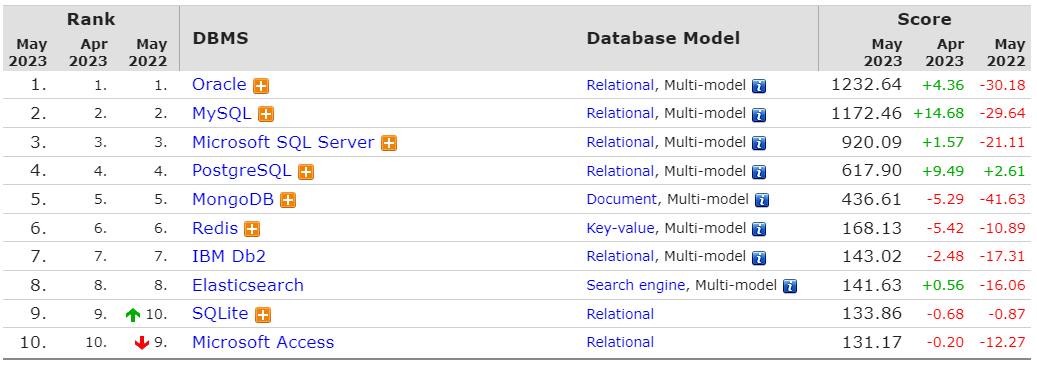
\includegraphics[width=14cm]{./assets/figures/MySQLPopularity.png}
        \caption{Popularité des différents SGBD dans le monde \label{MySQLPopularity.png}}
    \end{figure}
\end{center}
On voit également sur ce classement que les SGBD les deux permiers ont des scores assez similaires et ont tous deux de la marge sur leur concurrent qui occupe la troisième place. Je vais donc brièvement comparer Oracle avec MySQL.

\begin{center}
    \begin{figure}[H]%TODO : Changer la taille de cette image
        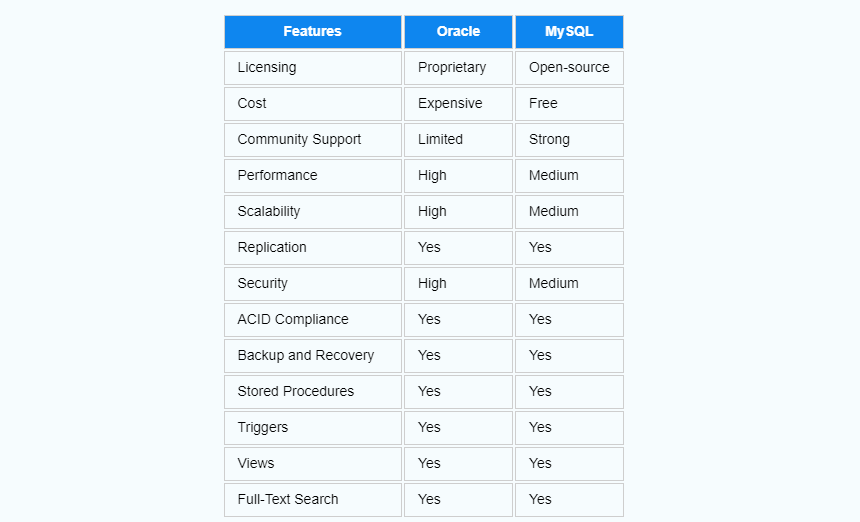
\includegraphics[width=\textwidth]{./assets/figures/OracleVsMySql.png}
        \caption{Comparaison entre Oracle et MySql \label{OracleVsMySql.png}}
    \end{figure}
\end{center}
Cependant comme montré dans l'article du site Integrate.io \cite{Integrate.io} les avantages sont minimes (des performances un peu meilleures et une sécuritée accrue). La licence Oracle étant cependant très onéreuse, ce dernier n'est pas un bon candidat dans le cadre de ce travail de Bachelor.

C'est pourquoi j'ai décidé de rester sur la version 8.0 de MySQL. Cependant, grâce au \emph{framework} Laravel il est extrêmement simple de changer de SGBD. En effet, il suffit de modifier le fichier de configuration. Si dans le futur, nous souhaitons pour une quelconque raison changer de SGBD, ce sera toujours possible et très facile.

\subsection{Laravel}
Laravel est un \emph{framework} \emph{open-source}, écrit en PHP, offrant une structure solide et élégante pour la création d'application et de site web. Le but principal de ce \emph{framework} est de simplifier la création et le développement d'application grâce à des fonctionnalités intégrées. Parmi ces fonctionnalités, on retrouve la gestion de routes, les sessions, l'authentification des utilisateurs ainsi que la gestion de la base de données.
Laravel fournit un ORM (\emph{Object Relational Mapping}), appelé Eloquent permettant de gérer toutes les interactions avec la base de données. Il permet également de choisir avec quel type de SGBD, nous souhaitons travailler et de changer ce dernier très rapidement grâce à des fichiers de configuration.
Il propose également un pattern architechtural très utilisé, le Modèle-Vue-Controller (MVC), que je vais rapidement expliquer.
\begin{center}
    \begin{figure}[H]%TODO : Changer la taille de cette image
        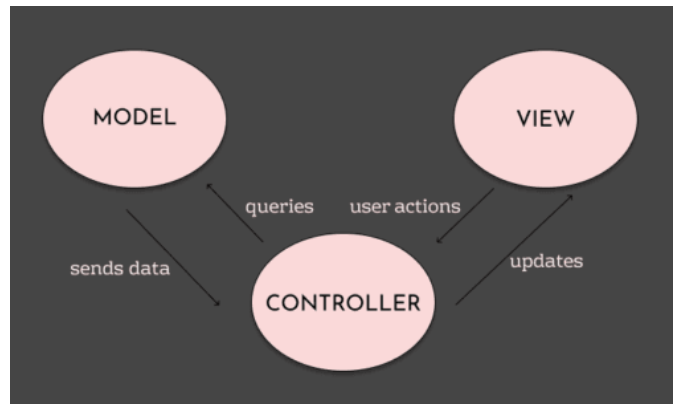
\includegraphics[width=\textwidth]{./assets/figures/MVCExplanation.png}
        \caption{Représentation du MVC \label{MVCExplanation.png}}
    \end{figure}
\end{center}

Sur cette capture, tirée du site Pusher \cite{MVC}, on peut voir les trois parties de ce système et comment elles interagissent.
\begin{itemize}
    \item Le Modèle est la partie responsable de la gestion des données ainsi que de la logique métier. C'est la seule partie du pattern qui interagit avec la base de données. Elle représente les structures de données, et fournit au \emph{Controller} des méthodes pour manipuler les données.
    \item La vue est la partie qui gère de l'interface utilisateur. Elle affiche les données et permet également de récupérer les informations saisies par l'utilisateur notamment au travers de formulaires.
    \item Le \emph{Controller} est la partie qui lie le Modèle et la Vue. Il réagit aux \emph{inputs} de l'utilisateur qui sont transmis par la Vue et va interroger, si nécessaire, le Modèle afin d'y mettre à jours ou récupérer des données. C'est également lui qui détermine quelle est la Vue à afficher à l'utilisateur. C'est le responsable de la logique de l'application.
\end{itemize}
Le MVC permet donc d'avoir une séparation distincte entre les différentes parties de notre application.

Un autre point fort de Laravel est sa gestion des \emph{middleware}. Un \emph{Middleware} est une sorte de filtre qui intervient lorsque les requêtes HTTP arrivent dans notre application. Cela permet notamment d'imposer qu'un utilisateur soit authentifié avant d'accéder à certaines ressources. Ils offrent donc un contrôle accru et centralisent la logique de certaines fonctionnalités.

Laravel est donc l'un des \emph{framework} les plus populaires, simple à prendre en main avec une documentation complète et mise à jour. Il est donc le candidat idéal pour ce projet. De plus, un changement de \emph{framework} imposerait une charge de travail supplémentaire bien trop conséquente.
Je vais donc utiliser la version 10 de Laravel.

\subsection{Vue.js}
Vue.js est un \emph{framework} JavaScript \emph{open-source}, populaire et polyvalent permettant de créer des interfaces utilisateur. Il est principalement utilisé pour le \emph{frontend} d'applications et peut facilement être ajouté à de gros projets. Il propose une approche basée sur les composants qui permettent de créer des portions de codes réutilisable. Grâce à une liaison bidirectionnelle entre les données et l'interface, Vue.js permet de synchroniser, en temps réel, les données entrées par l'utilisateur et leur affichage.

Ce qui permet à Vue.js d'être aussi performant est l'utilisation d'un \emph{DOM} virtuel. Le \emph{DOM (Document Object Model)} est une représentation hiérarchique d'un document HTML sous la forme d'un arbre. Il permet donc à des langages de programmation de modifier le style ou la forme de ce document. Cependant, à chaque changement, le navigateur va mettre à jour l'interface. Cela peut grandement impacter les performances si les modifications sont très fréquentes. C'est pourquoi Vue.js utilise un \emph{DOM} virtuel ou \emph{Virtual DOM}. Il s'agit d'une copie virtuelle stockée en mémoire du \emph{DOM} réel. Lors d'une mise à jour, les changements sont stockés dans le \emph{Virtual DOM}. Vue.js va ensuite comparer le \emph{Virtual DOM} avec le \emph{DOM} réel et n'appliquer que les changements nécessaires. Cela explique pourquoi ce \emph{framework} a des performances relativement élevées.

Pinia est le gestionnaire d'état conseillé pour la version 3 de Vue.js. Il permet de gérer l'état de l'application et de le partager entre les différents composants. Cet outil va nous être très utile au cours de ce projet.

Une autre fonctionnalité très importante de ce \emph{framework} est la capacité de créer des \emph{Singe Page Application} ou une application à page unique. Le concept derrière les SPA est que toute l'application est rendue sur une seule page. La SPA va initialement charger une page puis va dynamiquement changer son contenu en fonction des besoins et volontés de l'utilisateur. Cela permet une expérience utilisateur plus rapide et fluide qu'avec une application classique.

Les principaux concurrents du \emph{framework} Vue.js sont React et Angular. Selon un sondage réalisé par StackOverflow \cite{StackoverflowSurvey} en 2022, React est plus populaire que Vue.js et Angular.
\begin{center}
    \begin{figure}[H]%TODO : Changer la taille de cette image
        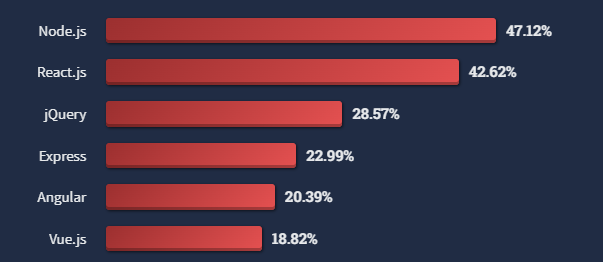
\includegraphics[width=\textwidth]{./assets/figures/VueVSReactVSAngular.png}
        \caption{Popularité des framework web \label{VueVSReactVSAngular.png}}
    \end{figure}
\end{center}

Comme Vue.js, React est un \emph{framework} javascript performant et dispose d'une communauté active. Il aurait été un bon choix de technologie pour ce projet, car plus utilisé dans l'industrie et disposant de plus d'utilisateurs.

Cependant, comme pour Laravel, un changement de \emph{framework} aurait imposé une charge de travail supplémentaire trop importante. De plus, Vue.js est plus simple à prendre en main et à utiliser que React. Il est donc mieux adapté à un projet de cette envergure. Je vais donc utiliser la version 3.0 de Vue.js.

\subsection{TailwindCSS}
TailwindCSS \cite{TailwindCSS} est un \emph{framework} CSS \emph{open-source} très simple à installer et utiliser. Il favorise la création rapide d'interfaces utilisateur personnalisées. Contrairement à son principal concurrent Bootstrap, TailwindCSS ne propose pas de composants prédéfinis. On y retrouve plutôt des classes utilitaires qui permettent de modifier rapidement le style d'un élément. Chaque classe est indépendante et ne représente qu'une fonctionnalité. Par exemple la classe "mb-4" permet d'ajouter une marge sur le bas d'un élément. Cela rend la personnalisation de l'interface utilisateur plus simple et plus rapide. On peut également créer ses propres classes utilitaires.

Un détail important de ce \emph{framework} est qu'il enlève tous les styles de base des navigateurs. Cela permet d'avoir une interface utilisateur cohérente sur tous les navigateurs.

Un autre point fort de ce TailwindCSS est sa communauté active. En effet, TailwindCSS dispose d'une documentation complète et de nombreux exemples.

Les raisons qui ont fait que j'ai choisi TailwindCSS sont sa simplicité d'utilisation, sa capacité de personnalisation. Bootstrap aurait été également un choix tout à fait valable. Cependant, pour avoir déjà travaillé avec ces deux \emph{framework}, j'ai une légère préférence pour TailwindCSS.

\subsection{Keycloak}
Keycloak \cite{Keycloak} est une solution \emph{open-source} de gestion d'identité et d'accès. Cela évite à notre application d'avoir à gérer les différents formulaires d'authentification, d'inscriptions ou de changement de mot de passe. Keycloak propose également une gestion des rôles et des permissions. Cela permet de définir des rôles pour les utilisateurs.

Dans le cadre de ce projet, tous les utilisateurs sont des membres de la HEIG-VD. Les deux choix que nous avions étaient d'utiliser Keycloak (le système de l'école) ou SWITCH edu-ID basé sur Shibboleth (actuellement utilisé dans le projet).

Le grand avantage de Keycloak est la maîtrise complète de l'outil par le service informatique de l'école. Cela permet une meilleure communication et entraide. De plus, Keycloak a déjà été utilisé sur plusieurs projets de l'école, donc sa mise en place sera simplifiée.
C'est pour ces raisons-là que j'ai décidé d'utiliser Keycloak.

\subsection{Github}
Github est une plateforme web de développement collaboratif basée sur Git. Elle facilite énormément la gestion de version de notre code source. De plus, elle favorise grandement la collaboration entre les différents développeurs. Github propose notamment des fonctionnalités de gestion de projet, permettant notamment des créer des tâches et de les assigner à des personnes. Ce qui aide à avoir une meilleure vue d'ensemble du projet.

Github permet également grâce à ses \emph{Github Actions} de créer des \emph{workflows CI/CD} qui permettent d'automatiser certaines tâches. Par exemple, on peut créer un \emph{workflow} qui va automatiquement lancer les tests unitaires à chaque modification du code qui sera poussé sur la plateforme. On peut également créer des \emph{Github Actions} qui vont déployer automatiquement notre application sur un serveur.

Github est la plateforme de gestion de version la plus populaire et la plus utilisée dans le monde. Selon les statistiques de l'article de Radix \cite{Radix}, Github aurait environ 56 millions d'utilisateurs contre 31 millions pour Gitlab. Avec son système de \emph{stars} et son côté social, Github est la plateforme idéale pour un projet open-source.

Toutes ces raisons font que Github est la plateforme de gestion de version choisie pour ce projet.
\newpage
\subsection{Récapitulatif des technologies}
Dans le tableau ci-dessous, vous pouvez trouver la liste de toutes les technologies qui sont utilisées dans le cadre de ce projet ainsi que leur version.
% Fais un tableau avec toutes les technologies utilisées dans le projet
\begin{table}[h]
    \begin{center}
        \caption{Technologies utilisées lors du projet \label{stack}}
        \begin{tabular}{|l|l|}
            \hline
            \textbf{Technologie} & \textbf{Version} \\
            \hline
            MySQL                & 8.0              \\
            \hline
            PHP                  & 8.2.6            \\
            \hline
            Composer             & 2.5.5            \\
            \hline
            Laravel              & 10               \\
            \hline
            Node                 & 18.15.0          \\
            \hline
            NPM                  & 9.5.0            \\
            \hline
            Vue.js               & 3                \\
            \hline
            Tailwind CSS         & 3.3.1            \\
            \hline
            WSL                  & 2                \\
            \hline
            Docker               & 20.10.22         \\
            \hline
            Ubuntu               & 22.04.2 LTS      \\
            \hline
            Keycloak local       & 21.1             \\
            \hline
            Github               & -                \\
            \hline
        \end{tabular}
    \end{center}
\end{table}

\chapter{Gestion du projet}
Cette section explique comment j'ai organisé mon travail et quels sont les outils que j'ai utilisés.

\section{Github}
Bien qu'un \emph{repository} Github existe déjà, j'ai fait le choix de partir d'une base vierge. J'ai donc créé un nouveau \emph{repository open source} ainsi que deux nouveaux projets pour le \emph{frontend} et le \emph{backend}. Il s'agit donc d'un \emph{mono-repo}, c'est quand un seul \emph{repository} contient plusieurs projets distinct. En effet, il me semblait plus simple de partir d'une base nouvelle et de réutiliser les éléments du projet existant au fur et à mesure. De plus, cela me permet d'avoir une meilleure maîtrise du projet dans son entièreté.

Une fois le travail terminé, il sera intéressant faire une \emph{Pull Request} sur le \emph{repository} de base afin de toujours avoir accès à toutes les versions et commit ce projet dans sa totalité.

Ce \emph{repository} est accessible \href{https://github.com/Marinlestylo/h-quiz}{en cliquant ici}. Il est structuré de la manière suivante :
\begin{itemize}
    \item \textbf{Un dossier "api-backend"} : contient le code du de notre API.
    \item \textbf{Un dossier "frontend"} : contient le code de l'interface utilisateur.
    \item \textbf{Un fichier .gitignore} : Explicite tous les fichiers qui ne doivent pas être poussés sur GitHub.
    \item \textbf{Un fichier README.md} : Explique les technologies et comment lancer le projet.
\end{itemize}

\subsection{README}
Comme mentionné dans le premier chapitre, le manque de documentation rend ce projet plus difficile à reprendre. C'est pourquoi j'ai décidé d'avoir un \emph{README} complet et précis permettant une reprise facilité du projet. On y trouve également des informations concernant le \emph{workflow} de ce projet ainsi que son déploiement.

% TODO : Expliquer que j'ai pas utilisé ça dans la section bilan
\subsection{User stories}
GitHub offre un système d'issue qui permet de signaler qu'une fonctionnalité doit être réalisée. Cela permet de garder une trace de ce qui doit être fait et de les marquer comme finie, une fois implémentée. Cela permet également de voir l'avancement du projet. Vous pouvez trouver la liste de toutes les issues ouvertes \href{https://github.com/Marinlestylo/h-quiz/issues}{ici}. Il est important de noter qu'à ce stade du projet, les issues ne sont pas encore toutes écrites.

GitHub nous offre également une vue d'ensemble de toutes ces issues. En effet, grâce à la fonctionnalité \emph{Projects}, nous pouvons créer des projets et y ajouter des issues. Avec la vue "tableau", nous avons une vue d'ensemble de toutes les issues et trois colonnes : \emph{To do}, \emph{In progress} et \emph{Done}. On peut donc savoir ce qui est en cours de réalisation. Ces fonctionnalités sont incroyablement utiles lorsqu'on travaille en équipe. Même si elles sont moins importantes quand on est seul sur un projet, cela nous permet de mesurer l'avancement du projet.

\subsection{Branches et commits}
Pour ce qui est de la gestion des branches, j'ai décidé de rester très simple et de n'utiliser que deux branches : \emph{main} et \emph{dev}. La branche \emph{main} est la branche principale. Elle doit être fonctionnelle à tout moment. C'est également la branche qui sera utilisée pour le déploiement du projet.

La branche \emph{dev}, quant à elle, sera celle où je vais développer les fonctionnalités. Lorsque plusieurs fonctionnalités sont implémentées et sont entièrement fonctionnelles, je fusionne les branches dans \emph{main}.

Je n'ai pas utilisé cette méthodologie de travail dès le début du projet. En effet, j'ai commencé par travailler directement sur la branche \emph{main} afin d'avoir une base solide pour le projet. Une fois que l'API, sa connexion avec Keycloak et les communications entre le \emph{frontend} et le \emph{backend} étaient fonctionnelles, j'ai créé la branche \emph{dev} et j'ai adopté cette méthodologie de travail.

Pour ce qui est des \emph{commits}, je me base sur les \emph{Conventional Commits} \cite{ConventionalCommits}. Plus particulièrement, tous mes \emph{commits} sont écrits en anglais et sont tous préfixés par un type.

Les types que j'utilise sont les suivants :
\begin{itemize}
    \item feat : Une nouvelle fonctionnalité a été ajoutée.
    \item fix : Une erreur a été corrigée.
    \item docs : La documentation a été modifiée.
    \item chore : Création d'un projet ou d'un dossier.
    \item refactor : Refactorisation d'une partie du code.
\end{itemize}

\section{Stratégie de refactoring}

Mon objectif principal était de reconstruire l'application de manière méthodique et progressive, tout en gardant une version fonctionnelle à tout moment. En effet, il était très important pour moi que l'application soit utilisable et puisse facilement être reprise à la fin de mon travail.

Pour cela, j'ai choisi de partir d'une base vierge et d'utiliser les dernières versions de Laravel et Vue.js, afin d'implémenter les fonctionnalités de manière itérative. Cette démarche m'a permis de m'inspirer du travail existant tout en bénéficiant des dernières fonctionnalités de ces technologies.

Une autre décision importante était de refactoriser simultanément le \emph{backend} et le \emph{frontend}. Cette approche me permet de tester directement l'interaction et le bon fonctionnement des deux parties ensemble. Cela évite également d'avoir à revenir sur du code écrit il y a plusieurs semaines, qui serait plus difficile à comprendre. Finalement, cela permet d'avoir une cohérence entre les deux parties et évite d'avoir une API qui contient des fonctionnalités qui ne sont pas utilisées par le \emph{frontend}.

%TODO ajouter la plannification


\chapter{Architecture et communication}
\section{Architecture de l'application}
Comme mentionné dans les chapitres précédents, l'application est divisée en deux parties bien distinctes : le \emph{frontend} et le \emph{backend}. Le \emph{frontend} est l'interface utilisateur. C'est ce que l'utilisateur voit et avec quoi il interagit. Le \emph{backend} est une API REST. C'est cette API qui permet la communication avec la base de données et la gestion des utilisateurs. La communication entre le \emph{frontend} et le \emph{backend} se fait via des requêtes HTTP.

On trouve également deux autres serveurs avec lesquels l'API communique. Le premier est Keycloak, qui permet l'authentification avec les comptes utilisateurs de l'école. Le second est un serveur de code qui permet aux utilisateurs de la plateforme d'écrire du code et de le compiler. La communication avec ces deux serveurs se fait également via des requêtes HTTP.

Vous trouverez un schéma expliquant cette architecture ci-dessous.

\fig[H, width=14cm]{Architecture de la plateforme}{Architecture.drawio}

\subsection{Communication standard}

Voici également un digramme de séquence expliquant ce qu'il se passe lorsque l'utilisateur veut accéder à une page qui affiche tous les quiz auxquels il a accès.

\fig[H, width=14cm]{Diagramme de séquence pour l'affichage de tous les quiz}{ArchitectureSequence.drawio}

Il est important de noter que dans ce diagramme, il n'y a pas encore de notion d'authentification. Cette notion sera expliquée dans la section suivante.

\section{Authentification}
Dans cette sous-section, je vais expliquer comment a été gérée l'authentification via Keycloak.

\subsection{Processus d'authentification}
Pour implémenter l'authentification avec Keycloak, il y avait deux possibilités envisageables. La première option était de gérer la connexion avec Keycloak depuis le \emph{frontend}. Cela implique que Keycloak retourne un \emph{token} d'authentification au \emph{frontend} et que ce dernier l'envoie à l'API à chaque requête. L'API vérifie ensuite la validité du \emph{token} auprès du serveur Keycloak et renvoie une réponse en conséquence. Cette approche est parfaitement viable et est utilisée dans d'autres projets de la HEIG-VD.

Le point faible de cette approche est que le \emph{frontend} et le \emph{backend} doivent tous les deux travailler avec Keycloak. Cela implique que si on veut changer de fournisseur d'identité, il faut modifier les deux parties de l'application.
C'est pour cette raison qu'une autre approche a été mise en place où uniquement le \emph{backend} travaille avec Keycloak.

Le digramme de séquence qui suit explique de façon détaillée quel est le processus d'authentification. À noter que le processus de déconnexion est similaire.
\fig[H, width=14cm]{Digramme de séquence pour l'authentification d'un utilisateur}{connexionFlow.drawio}

Même si c'est un processus assez long et complexe, il a le grand avantage que le \emph{frontend} n'a aucune connexion directe avec le serveur d'authentification. Si nous décidons dans le futur de changer de fournisseur d'identité, il ne faudra modifier que le \emph{backend}.

\subsection{Communication avec authentification}

\fig[H, width=14cm]{Accès à une ressource sans être authentifié}{forbidden401.drawio}

Ce diagramme illustre ce qu'il se passe lorsque l'utilisateur veut accéder à une page qui nécessite une connexion, mais que ce dernier n'est pas encore authentifié. Il reçoit une erreur 401 \emph{Unauthorized}. C'est l'erreur standard pour indiquer qu'une ressource est protégée et que l'utilisateur doit être authentifié pour y accéder. A noter qu'un mécanisme similaire sera mis en place si un utilisateur authentifié tente d'accéder à une ressource qui lui est interdite. Par exemple, un étudiant qui tenterait d'accéder à une ressource réservée aux enseignants. L'erreur qu'il recevrait serait ici une erreur 403 \emph{Forbidden}.

\chapter{Base de données}
Cette section montre le contenu initial de la base de données au début du projet, ainsi que les ajustements et ajouts effectués.

\section{Base de données initiale}

Voici le schéma de la base de données lors de la reprise du projet :

\begin{figure}[H]
    \begin{center}
        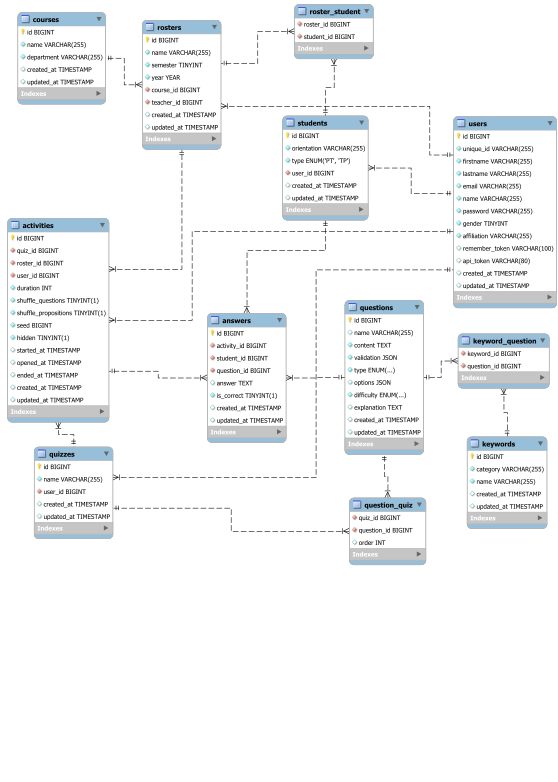
\includegraphics[width=14cm]{\assetsdir/diagramBaseDB.svg.pdf}
    \end{center}
    \caption[Diagramme de la base de données initiale]{\label{assembly}Diagramme de la base de données initiale}
\end{figure}

Il est donc nécessaire de modifier cette base de données afin qu'elle puisse répondre aux nouveaux besoins de l'application. De plus, quelques modifications seront effecutées afin d'éviter la redondance de données. Les détails de ces ajustements sont présentés dans les sections suivantes.

\section{Modifications apportées aux tables existantes}

\subsection{Table "users"}
Plusieurs modifications ont été effectuées dans cette table. Notamment, le champ "name" qui a été supprimé, car il était une concaténation des champs "firstname" et "lastname". Il convient donc de l'enlever afin d'éviter la redondance de données. Le champ \emph{unique\_id} devient \emph{keycloak\_id} et permet de savoir lors de la connexion si un utilisateur possède déjà un compte sur l'application ou si l'on doit le créer. Les champs \emph{password} et \emph{api\_token} sont quant à eux supprimés car plus nécessaire.

\subsection{Table "quizzes"}
La seule modification apportée à cette table est l'ajout d'un champ \emph{type} qui est une \emph{enum} comprenant les valeurs \emph{quiz} et \emph{exam}. Ce champ permet de différencier les quiz des examens.

\subsection{Table "questions"}
Le champ \emph{type} de cette table a été étendu afin d'ajouter la valeur \emph{long-answer} aux quatre autres valeurs déjà existantes (\emph{"short-answer", "fill-in-the-gaps", "multiple-choice"} et \emph{"code"}). Cette valeur permet de différencier les questions à développement des questions à réponse courte. L'ajout d'un \emph{user\_id} permet de connaître le créateur de la question et de restreindre la modification de la question uniquement à ce dernier. Cet ajout, lié au nouveau champ \emph{is\_public} permet de créer des questions privées qui ne pourront pas être utilisées par d'autres professeurs dans leurs quiz. De plus, l'ajout d'un champ concernant la visibilité de la question sera utile pour savoir quelles questions peuvent être sélectionnées dans le mode \emph{drill}. Enfin, l'ajout du champ \emph{points} permet d'attribuer un nombre de points à chaque question, ce qui est essentiel pour calculer le nombre total de points d'un examen ou d'un quiz.

\subsection{Table "answers"}
Un champ \emph{points} a également été ajouté à cette table, permettant de d'attribuer un certain nombre de points à la réponse d'un élève. Ce champ est utilisé pour calculer le nombre de points obtenus par un élève à un examen ou un quiz.

\section{Intégrité des données}
Avec l'ajout de travaux écrits sur la plateforme, la question de l'intégrité des données se pose. En effet, puisque les questions sont modifiables par leur créateur, il est alors possible qu'un enseignant modifie une question d'examen après que ce dernier se soit déroulé. Ce qui aurait des conséquences directes sur les réponses des élèves. Pour éviter cela, deux solutions sont envisagées.

La première solution consiste à fournir un \emph{hash} de l'examen et de toutes ses questions que les étudiants pourront comparer lors de la correction. Cette solution présente comme avantage la facilité de mise en place, mais a un énorme défaut. En effet, un examen peut contenir des questions créées par d'autres enseignants. Ces derniers pourraient donc modifier leurs questions indépendamment de la volonté de l'enseignant responsable de l'examen. Suite à la modification, la comparaison des deux hash nous dirait donc que l'examen a bien été modifié mais il serait impossible de savoir à quel point et que faire pour corriger cela.

La deuxième solution, plus compliquée à mettre en place, consiste à copier les questions de l'examen dans une table distincte. Cela va créer une certaine redondance des données, mais c'est la solution qui semble être le mieux adapté à notre situation. La copie des questions se ferait lors du lancement du quiz de type examen. Ensuite, lors de l'examen, l'application ira lire les questions dans cette table à part. Ainsi, si un enseignant modifie une question après le début de l'examen, cela n'aura aucune conséquence sur les réponses des élèves. Pour éviter au maximum la redondance de données, on ne copiera que les questions d'un quiz de type examen et non les questions des quiz normaux.

Cette deuxième solution semble donc être la plus adaptée à notre situation. Elle permet de garder l'intégrité des données tout en évitant au maximum la redondance de données. Cependant si une personne à accès à la base de données, rien ne l'empêchera de modifier les questions de l'examen. C'est pourquoi une combinaison des deux solutions est la solution choisie.

\section{Ajout de tables}

\subsection{Table activity\_student}
Cette table a été créée dans le but de savoir si l'étudiant a rendu un examen ou non. Lorsqu'un élève termine un quiz en avance, il peut le rendre. Cependant, s'il retourne sur l'activité, il peut continuer de répondre aux questions. Grâce à l'ajout de cette relation, il est désormais possible de savoir si l'étudiant effectivement rendu son examen, permettant ainsi de limiter son accès le cas échéant.

\subsection{Table exam\_questions}
Comme expliqué dans la section sur l'intégrité des données, cette table permet de faire une copie des questions d'un examen. Certains champs n'ont pas été copiés dans cette nouvelle table. En effet, des champs tels que \emph{is\_public} ou \emph{user\_id} ne sont pas pertinent à dupliquer, car leur modification n'aura pas d'impact sur les réponses des élèves. On peut noter que le champ \emph{user\_id} de la table \emph{exam\_questions} aurait également pu être abandonné. Actuellement, le créateur de la question ne peut pas être modifié via l'application. Cela pourrait cependant être une fonctionnalité supplémentaire. C'est pour garder l'information sur le "propriétaire" de la question que ce champ a été conservé.

\subsection{Table drills}
Cette table a été créée dans le but de gérer le mode \emph{drill} de l'application. Une section du chapitre suivant est dédiée à cette fonctionnalité, c'est pourquoi il n'y a pas le détail sur les champs secondaires. Les trois clés étrangères \emph{student\_id}, \emph{question\_id} et \emph{keyword\_id} sont essentielles pour récupérer toutes les questions publiques avec un mot-clé spécifique pour un étudiant donné. Ces clés permettent de savoir si l'étudiant a déjà répondu à une question avec un mot-clé particulier, afin d'adapter les prochaines occurrences en fonction de ses résultats.

\subsection{Diagramme de modification de la base de données}
Pour des raisons de clarté, ce schéma montre toutes les tables, mais n'affiche que les nouvelles relations. Un diagramme complet se trouve à la section suivante.

\begin{figure}[H]
    \begin{center}
        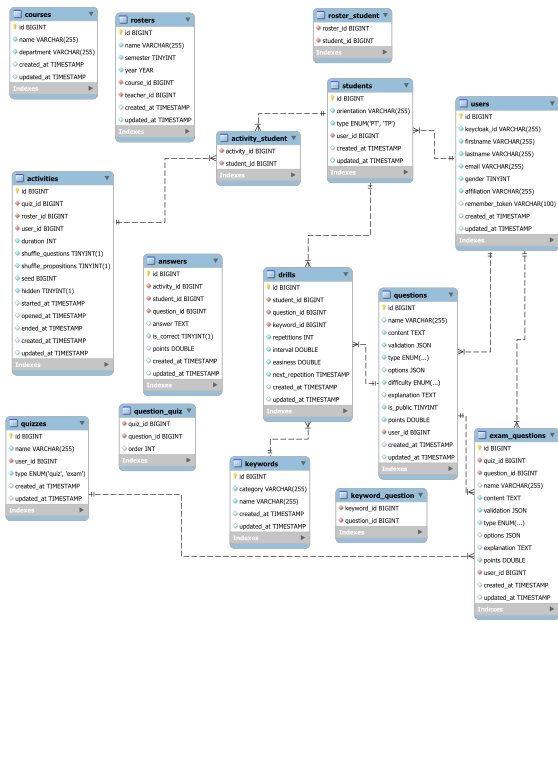
\includegraphics[width=14cm]{\assetsdir/diagramDBAdded.svg.pdf}
    \end{center}
    \caption[Diagramme des modifications de la base de données]{\label{assembly}Diagramme des modifications de la base de données}
\end{figure}

\section{Base de données finale}
Voici un schéma complet de la base de données après les modifications appliquées :
\begin{figure}[H]
    \begin{center}
        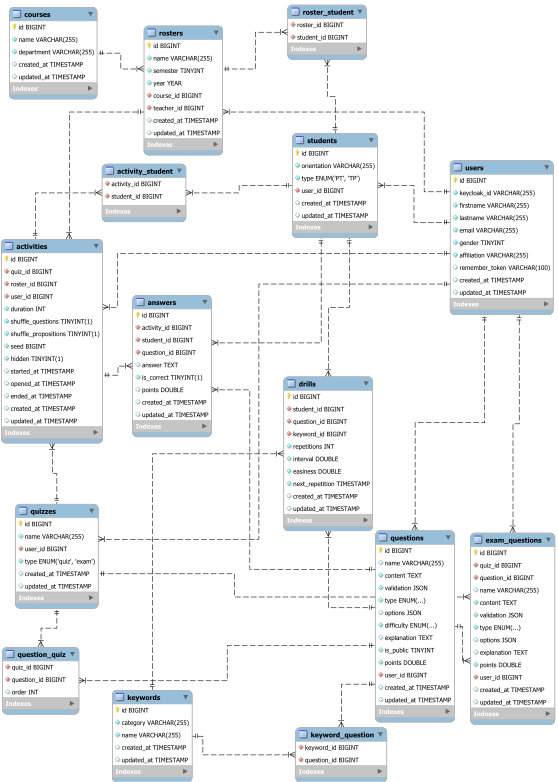
\includegraphics[width=14cm]{\assetsdir/digramDB.svg.pdf}
    \end{center}
    \caption[Diagramme de la base de données finale]{\label{assembly}Diagramme de la base de données finale}
\end{figure}

\chapter{Réalisation du Backend}
\section{Keycloak}
Pour l'implémentation, j'ai utilisé une librairie nommée Socialite Providers \cite{SocialiteProviders}. Cette librairie permet de gérer l'authentification avec Keycloak dans Laravel. Je me suis également inspiré du projet \emph{Fablab-name} \cite{FablabName} du Professeur Yves Chevallier qui utilise également cette librairie.

En premier lieu, j'ai dû modifier le fichier \emph{app/providers/EventServiceProvider.php} afin d'y rajouter un \emph{event listener}.
\begin{listing}[H]
    \inputminted{php}{assets/code/serviceProviderkeycloak.php}
    \caption{EventServiceProvider \label{serviceProviderkeycloak}}
\end{listing}

Suite à cela, il faut créer deux routes pour le \emph{login} et une pour le \emph{logout}. Ces routes sont définies dans le fichier \emph{routes/api.php}.

\begin{listing}[H]
    \inputminted{php}{assets/code/routeKeycloak.php}
    \caption{Routes pour l'authentification Keycloak \label{routeKeycloak}}
\end{listing}

On peut voir que la route de déconnexion n'est accessible que par un utilisateur connecté pour éviter des erreurs.

Finalement, j'ai créé un \emph{KeycloakController} qui s'occupe de gérer la logique de l'authentification. Ce fichier se trouve dans \emph{app/Http/Controllers/KeycloakController.php}.

\begin{listing}[H]
    \inputminted{php}{assets/code/keycloakController.php}
    \caption{KeycloakController \label{keycloakController}}
\end{listing}

Dans ce \emph{Controller}, on va s'intéresser à trois méthodes :
\begin{itemize}
    \item \emph{redirect} : Cette méthode redirige l'utilisateur vers la page de login de Keycloak.
    \item \emph{callback} : Cette méthode est appelée une fois que l'utilisateur s'est authentifié avec succès. Elle va ensuite créer ou modifier l'utilisateur dans la base de données. Finalement, elle va rediriger l'utilisateurs vers le \emph{frontend}.
    \item \emph{logout} : Cette méthode va déconnecter l'utilisateur de Keycloak et le rediriger vers le \emph{frontend}.
\end{itemize}

La dernière modification est faite dans le fichier \emph{app/Http/Middleware/Authenticate.php}. C'est à cet endroit que l'on va vérifier si l'utilisateur est authentifié. Si ce n'est pas le cas, on retourne une erreur 401.

\begin{listing}[H]
    \inputminted{php}{assets/code/authenticate.php}
    \caption{Renvoie de l'erreur 401 \label{authenticate}}
\end{listing}


\subsubsection{Modification de la base de données}
Suite à cette implémentation, il m'a fallu faire des modifications dans la table \emph{users} de la base de données. En effet, les champs suivants ont été supprimés :
\begin{itemize}
    \item \emph{name} : Ce champ est une concaténation du nom et prénom de l'utilisateur. Il a donc été supprimé car ces informations sont redondantes.
    \item \emph{password} : Ce champ n'existe tout simplement plus, car nous ne stockons pas le mot de passe du Keycloak.
    \item \emph{api\_token} : Ce champ n'existe plus.
\end{itemize}

De plus, j'ai rajouté le champ \emph{keycloak\_id} qui contient l'identifiant unique de l'utilisateur dans Keycloak. Ce champ est utilisé pour vérifier si l'utilisateur existe déjà dans la base de données. Si c'est le cas, on met à jour les informations de l'utilisateur. Sinon, on crée un nouvel utilisateur.

\chapter{Réalisation du Frontend}
\section{Communication avec le backend}
La communication entre le \emph{frontend} et le \emph{backend} s'effectue à l'aide de requêtes \emph{fetch}. Étant donné que de nombreux composants du \emph{frontend} ont besoin de communiquer avec le \emph{backend}, un fichier \emph{utils.js} a été dans le dossier \emph{src} contenant une fonction permettant de faire des requêtes \emph{fetch} à l'API. Cette approche de centralisation permet de factoriser le code et de faciliter d'éventuelles modifications ultérieures.


\begin{listing}[H]
    \inputminted{js}{assets/code/communcation.vue}
    \caption{Communication avec le backend}
\end{listing}

Cette fonction prend en paramètre une \emph{url}, et un objet contenant les paramètres de la requête. Son objectif est de fournir une approche unifiée pour différentes requêtes HTTP telles que \emph{GET, POST, PATCH, PUT} et \emph{DELETE}. Il est également possible de rajouter des données au format \emph{JSON} dans le corps de la requête. On y voit également deux constantes qui sont définies dans le fichier \emph{.env} du projet. Cela permet de changer l'adresse du backend sans avoir à changer le code.

Pour mieux illustrer son utilisation, un exemple concret sera présenté dans la section \emph{Store} ci-dessous.

\section{Store}
Les stores jouent un rôle essentiel dans cette partie du projet. Ils permettent de stocker des données directement dans le \emph{frontend} de l'application, évitant ainsi des requêtes trop fréquente à l'API qui auraient un impact négatif sur les performances de l'application. De plus, les stores permettent de centraliser les différents appels à l'API, ce qui contribue à une meilleure organisation et factorisation du code.

Un exemple très parlant de leur utilité est la gestion des informations d'un utilisateur connecté. S'il était nécessaire de faire un appel supplémentaire à l'API à chaque changement de vue ou de composant, cela serait coûteux en performance.
Voici un extrait de code du \emph{store user} :

\begin{listing}[H]
    \inputminted{js}{assets/code/userStore.js}
    \caption{Store utilisateur}
\end{listing}

On peut voir l'import du fichier \emph{utils.js} ainsi que l'utilisation de la fonction \emph{fetchApi}.
L'objet \emph{user} est déclaré pour stocker les informations de l'utilisateur connecté.

Un point intéressant est que la fonction \emph{fetchUser} vérifie si l'objet \emph{user} est vide avant de faire un appel à l'API. Si les informations sont déjà en possession, un appel à l'API est donc évité. Lors de l'utilisation de cette fonction dans les composants et vues, on n'a pas à se soucier de savoir si l'appel est redondant. Cela permet de grandement simplifier le code.

La fonction \emph{logout} permet de déconnecter l'utilisateur. Cette fonction ne fait que supprimer l'objet \emph{user} du \emph{store}, car c'est l'API qui gère la connexion ainsi que la déconnexion.

Finalement, en bas du fichier, on peut voir un \emph{return} qui expose les fonctions et variables du \emph{store} aux composants et vues.

Tous les \emph{stores} de ce projet suivent une structure similaire à celle-ci.

\section{Middleware}
L'un des gros défauts de l'ancien \emph{fontend} est qu'il n'y avait aucune logique empêchant un utilisateur non connecté d'accéder à des pages nécessitant une connexion. Cette lacune pouvait entraîner toutes sortes de bugs et d'incohérences dans le fonctionnement de l'application. De plus, l'utilisateur non connecté ou ne disposant pas des droits nécessaires ne pouvait pas utiliser ces pages correctement. Ce qui constitue donc un problème autant d'un point de vue sécurité que de l'expérience utilisateur. Il est donc impératif de le régler.

Pour palier à cela, deux \emph{middleware} ont été mis en place en se basant sur cet article \cite{middlewareVuejs}.

Dans un premier temps, il faut créer un fichier \emph{auth.js} dans le dossier \emph{middleware} du projet. Il y a également un \emph{middleware} pour les enseignants qui a été créé mais son code, très similaire à celui-ci, ne sera pas montré.

\begin{listing}[H]
    \inputminted{js}{assets/code/auth.js}
    \caption{Middleware authentication}
\end{listing}
Ce code présente une fonction qui utilise le \emph{store} pour vérifier si l'utilisateur est connecté. Si ce n'est pas le cas, on le redirige vers la vue \emph{root}, sinon on le laisse accéder à la page demandée.

Ensuite, un autre fichier nommé \emph{middleware-pipeline.js} est créé dans le même dossier.
\begin{listing}[H]
    \inputminted{js}{assets/code/middlewarePipeline.js}
    \caption{Middleware pipeline}
\end{listing}

Cette fonction prend un tableau de \emph{middleware} en paramètre et traverse ce tableau en appliquant chacun des \emph{middleware}. Si l'un des \emph{middleware} bloque l'accès à l'utilisateur, le processus se termine et l'utilisateur est redirigé vers la page \emph{root}. Si tous les \emph{middleware} autorisent l'accès, alors l'utilisateur est autorisé à atteindre cette ressource.


Finalement, dans le fichier \emph{index.js} du dossier \emph{router}, on ajoute ce code :

\begin{listing}[H]
    \inputminted{js}{assets/code/beforeEachRoute.js}
    \caption{Actions effecutées avant chaque route}
\end{listing}

Ceci permet de définir une action qui sera exécutée avant chaque accès à une route.

On peut ajouter un certain \emph{middleware} à la déclaration d'une route de la manière :

\begin{listing}[H]
    \inputminted{js}{assets/code/route.js}
    \caption{Utilisation du middleware}
\end{listing}


\section{Changements graphiques}
Suite à la refonte du \emph{frontend} avec TailwindCSS, de nombreux changements ont été apportés. Bien que l'interface ait été modifiée, beaucoup de pages sont restées relativement similaires. Seuls les changements les plus importants seront présentés ici.

\subsection{Popup d'information}
Un problème majeur de l'ancien \emph{frontend} était l'absence de \emph{popup} d'information informant l'utilisateur du succès ou de l'échec d'une action. Parfois, même si tout fonctionnait comme prévu, en l'absence d'information visuelle, l'utilisateur pouvait penser que l'action n'avait pas été effectuée.
C'est pourquoi une popup d'information a été ajoutée. Il permet d'afficher un message à l'utilisateur et est utilisé dans la plupart les composants et vues du projet.

Voici un exemple d'utilisation de cette \emph{popup} :
\begin{center}
    \begin{figure}[H]
        
\includegraphics[width=\textwidth]{./assets/figures/validationPopup.png}
        \caption{Popup d'information}
    \end{figure}
\end{center}

Une variante de cette même \emph{popup} est utilisée pour signaler les erreurs :
\begin{center}
    \begin{figure}[H]
        
\includegraphics[width=\textwidth]{./assets/figures/errorPopup.png}
        \caption{Popup d'erreur}
    \end{figure}
\end{center}

\subsection{Menu}
Le menu de l'ancienne application n'étant pas très intuitif et ne s'adaptait pas à au rôle de l'utilisateur. Il s'adapte désormais au rôle de ce dernier et comporte des menu déroulant.

\begin{center}
    \begin{figure}[H]
        
\includegraphics[width=\textwidth]{./assets/figures/basicNav.png}
        \caption{Menu utilisateur non connecté}
    \end{figure}
\end{center}

\begin{center}
    \begin{figure}[H]
        
\includegraphics[width=\textwidth]{./assets/figures/teacherNav.png}
        \caption{Menu enseignant}
    \end{figure}
\end{center}

\begin{center}
    \begin{figure}[H]
        
\includegraphics[width=\textwidth]{./assets/figures/studentNav.png}
        \caption{Menu élève}
    \end{figure}
\end{center}

\subsection{Documentation}
Afin de faciliter la compréhension de la création de quiz et de questions, une page supplémentaire dédiée à la documentation a été ajoutée.

\begin{center}
    \begin{figure}[H]
        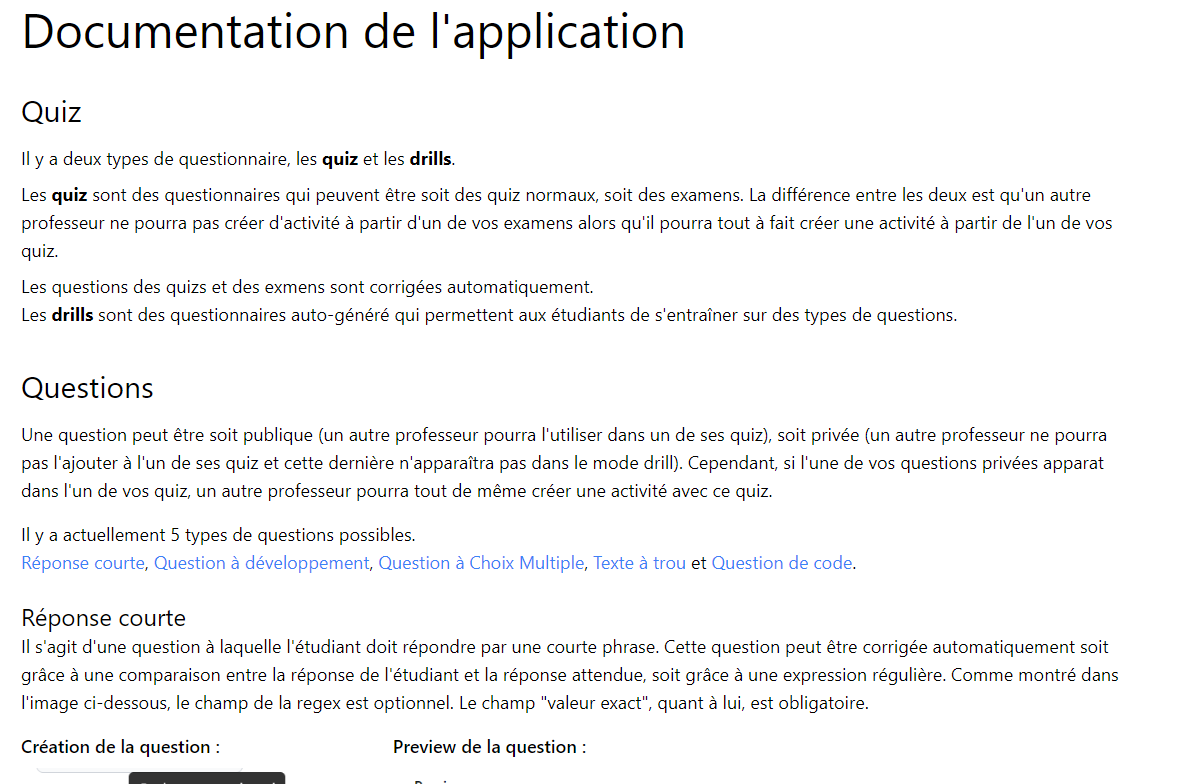
\includegraphics[width=\textwidth]{./assets/figures/documentation.png}
        \caption{Page de documentation de l'application}
    \end{figure}
\end{center}

\subsection{Page 404}
Une page par défaut a été mise en place lorsque l'utilisateur entre une \emph{URL} qui ne correspond à aucune vue existante.

\begin{center}
    \begin{figure}[H]
        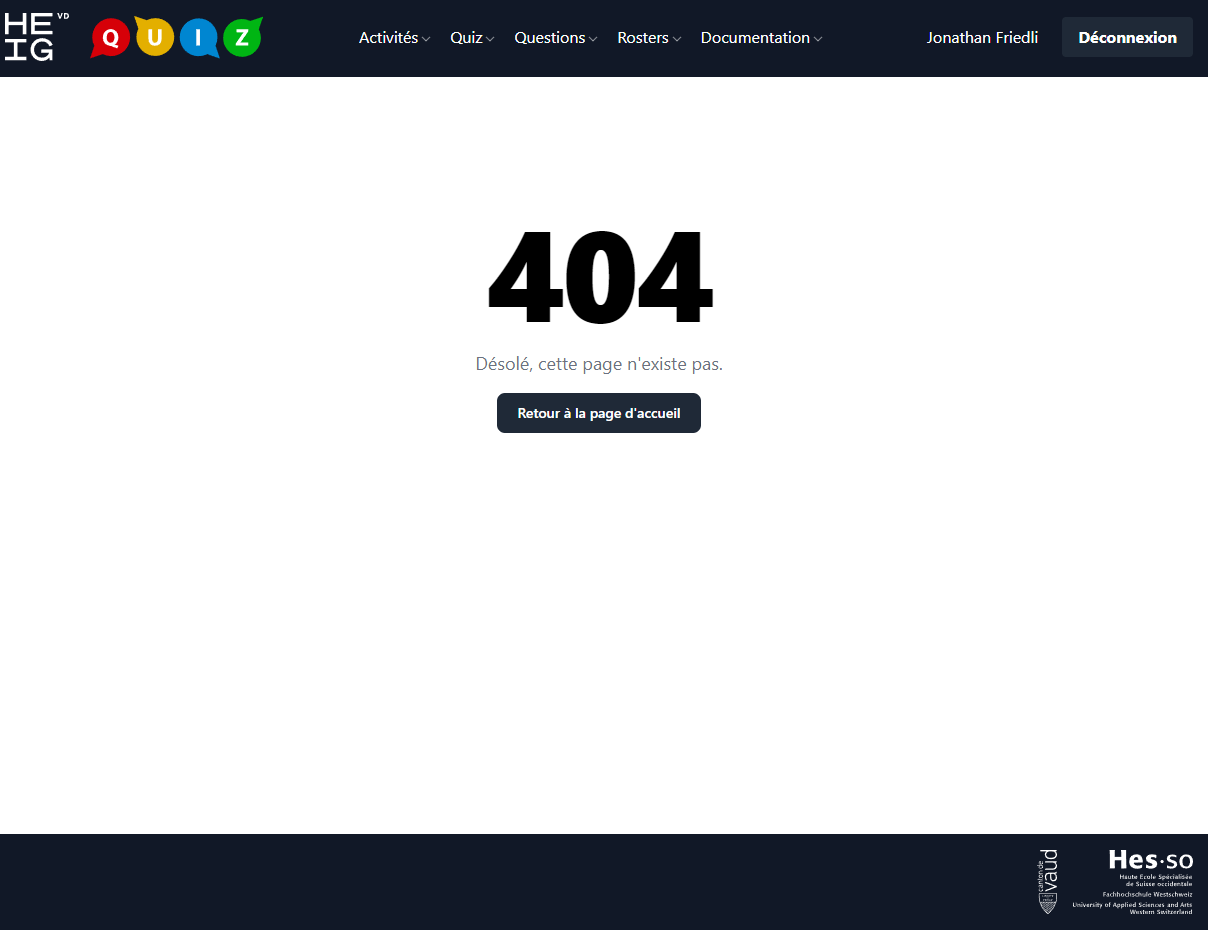
\includegraphics[width=\textwidth]{./assets/figures/page404.png}
        \caption{Page non trouvée}
    \end{figure}
\end{center}


\section{Compilation de code}
La fonctionnalité permettant de compiler le code a été réalisée dans un composant réutilisable. Ce qui permet d'utiliser cette dernière à la fois dans la \emph{preview} lors de la création ou modification, mais également lors d'un quiz, d'un examen ou d'un \emph{drill}.
Voici à un aperçu du fonctionnement :
\begin{center}
    \begin{figure}[H]
        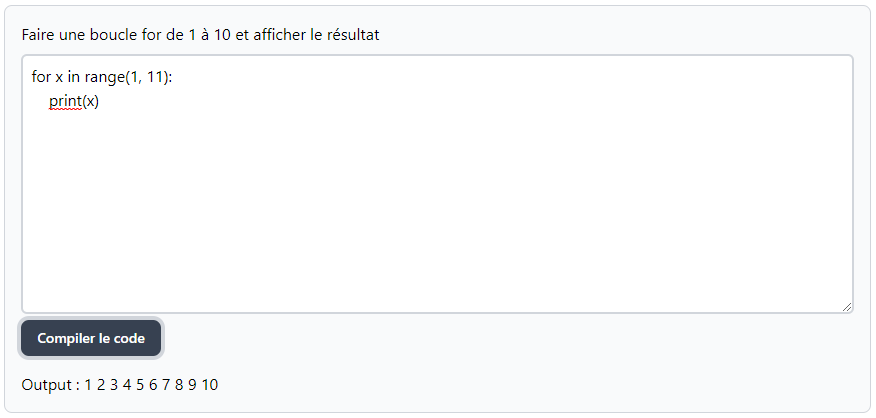
\includegraphics[width=\textwidth]{./assets/figures/codeCompilation.png}
        \caption{Compilation de code}
    \end{figure}
\end{center}

En cas d'erreur dans le code saisi, le comportement est également géré de manière appropriée :
\begin{center}
    \begin{figure}[H]
        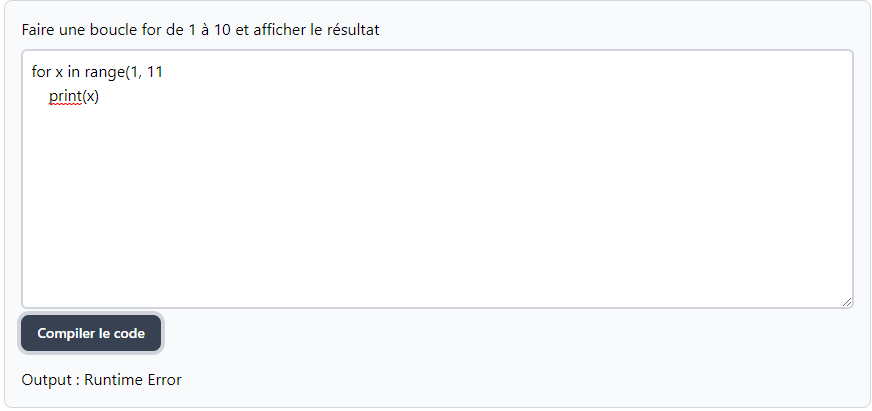
\includegraphics[width=\textwidth]{./assets/figures/codeCompilationError.png}
        \caption{Compilation de code avec erreur}
    \end{figure}
\end{center}

\section{Quiz et examens}
Les quiz et les examens sont entièrement fonctionnels. Ils partagent tous deux le même composant. La différence est que si un étudiant rend un examen en avance, il ne pourra plus y accéder. Tandis que si ce dernier rend un quiz en avance, il peut toujours revenir et modifier ses réponses. Cette mesure a été mise en place pour prévenir toute tentative de triche.

De plus, un détail important à noter est que les questions se chargent au fur et à mesure. Lorsqu'un étudiant accède à une question pour la première fois, l'application fait une requête à l'API afin de récupérer les informations. Ensuite, ces dernières sont stockées dans le \emph{store} de l'activité afin de rendre l'application la plus fluide possible.

Exemple de quiz :

\begin{center}
    \begin{figure}[H]
        
\includegraphics[width=\textwidth]{./assets/figures/quizExample.png}
        \caption{Exemple de quiz}
    \end{figure}
\end{center}

\section{Drill}
Le mode \emph{drill} se décompose en deux parties. Tout d'abord, l'utilisateur sélectionne un mot-clé parmi les choix proposés.


\begin{center}
    \begin{figure}[H]
        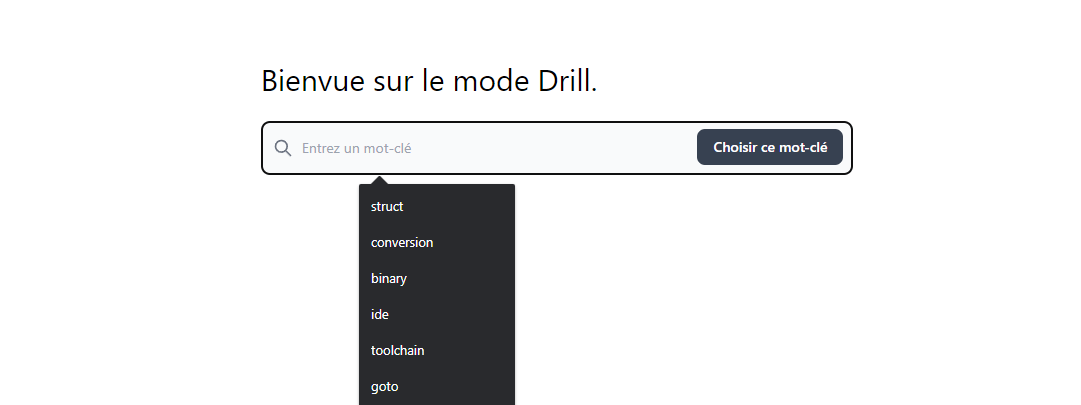
\includegraphics[width=\textwidth]{./assets/figures/drill1.png}
        \caption{Choix du mot-clé}
    \end{figure}
\end{center}

Une fois cette étape effectuée, l'utilisateur est redirigé sur une nouvelle page contenant uniquement des questions publiques associées au mot-clé choisi.
Un chronomètre démarre alors et l'utilisateur doit répondre à la question.
\begin{center}
    \begin{figure}[H]
        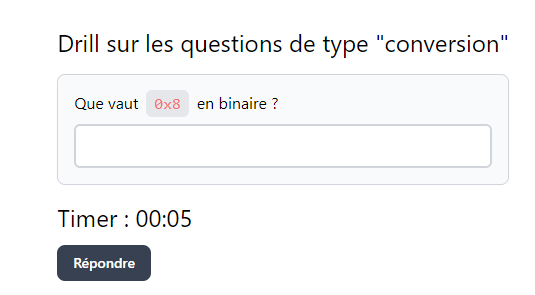
\includegraphics[width=\textwidth]{./assets/figures/drill2.png}
        \caption{Question en mode drill}
    \end{figure}
\end{center}

Une fois sa réponse validée, l'utilisateur peut voir la bonne réponse et l'application indique si sa réponse a été acceptée ou non.

\begin{center}
    \begin{figure}[H]
        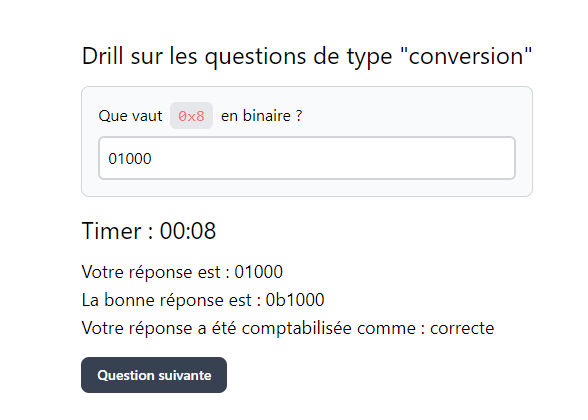
\includegraphics[width=\textwidth]{./assets/figures/drill3.png}
        \caption{Réponse du mode drill}
    \end{figure}
\end{center}

En fonction de sa réponse, cette question reviendra plus ou moins vite. L'utilisateur peut alors cliquer sur le bouton "question suivante" pour continuer le \emph{drill}.
Une fois que l'utilisateur a répondu à toutes les questions, il n'est pas obligé d'attendre le jour suivant pour continuer de répondre aux questions. Ce choix a été fait afin d'éviter que l'utilisateur ait à attendre un où plusieurs jours pour ne répondre qu'a une ou deux questions. Ce qui pourrait être le cas si seulement une dizaine question sont affiliés à certains mots-clés spécifiques.

\chapter{CI/CD et déploiement}
\section{Déploiement}
Pour s'assurer du bon fonctionnement du projet et vérifier que les fonctionnalités ne se limitent pas à un environnement local, il est essentiel de le déployer. Le projet est actuellement déployé à l'adresse suivante : \url{https://h-quiz.heig-vd.site/}. À noter que ce nom de domaine n'appartient pas à la HEIG-VD. Actuellement, le site est utilisable et il est possible de s'y connecter avec son compte de la HEIG-VD.

Cependant, pami les informations transmises par le serveur keycloak ne permettant pas de différencier un étudiant d'un professeur. Actuellement, chaque utilisateur est considéré comme un enseignant. Une demande a été faite afin que cette information puisse être ajoutée. Si cela ne s'avère pas réalisable, une autre approche serait de maintenir une liste d'e-mails appartenant aux enseignants et au personnel de l'école. A chaque connexion, l'application vérifierait ainsi si l'utilisateur est dans la liste.

\section{CI/CD}
\subsection{Tests}
Dans le cadre de ce projet, seuls les tests du \emph{backend} de l'application ont été effectués. Bien que des tests du \emph{frontend} soient envisageables, il a été jugé que cela nécessiterait un temps trop considérable.

Laravel propose deux types de tests bien distincts : les \emph{Unit test} et les \emph{feature test}. Les premiers se concentrent sur de toutes petites fonctionnalités du code, comme des méthodes. En revanche, les \emph{feature tests} permettent de tester des parties plus vastes du code, comme une route de l'API. Dans ce projet, les \emph{feature tests} ont été privilégiés, étant donné que l'API ne présente pas d'unités de code particulièrement adaptées au \emph{unit testing}.

Des tests ont donc été rédigés afin de tester le comportement général de l'application. Principalement pour tester l'accès à des routes protégées mais également afin de tester la logique de certains \emph{Controller}. Il faudrait cependant ajouter des tests afin que tous les \emph{Controller} soient tester.

\subsection{Github actions}
Grâce aux \emph{github actions}, il est possible de lancer automatiquement les tests de Laravel après un \emph{push} ou une \emph{Pull request} sur certaines branche. Cette approche garantit la détection rapide de toute modification susceptible de compromettre le bon fonctionnement de l'application. De plus, lors de travaux d'équipes, ce genre d'outils est indispensable.

Voici la \emph{github action} qui lance les tests de manière automatique :

\begin{listing}[H]
    \inputminted{yaml}{assets/code/laravelCI.yaml}
    \caption{Github action lançant les tests automatiques}
\end{listing}

Dans les première lignes, on peut voir que ces tests ne sont effectués que lors d'un \emph{push} sur la branche \emph{main} ou d'une \emph{Pull request} sur la branche sur cette dernière. Cette approche vise à empêcher tout code défaillant d'être poussé sur la branche principale. Ensuite, les dépendances sont installées, puis une base de données sqlite est configurée et les tests sont exécutés.
Cette \emph{GitHub Action} simple, mais efficace permet de vérifier que l'application reste fonctionnelle lors de l'intégration de nouvelles fonctionnalités dans la branche \emph{main}.

Le pipeline de \emph{CI/CD} comprend également une deuxième \emph{github action} plus complexe qui gère le de \emph{build} le déploiement automatique sur un serveur de production.

\begin{listing}[H]
    \inputminted{yaml}{assets/code/deployCD.yaml}
    \caption{Déploiement automatique}
\end{listing}

Cette \emph{github action} n'est effectuée uniquement lors de \emph{push} sur la branches \emph{main}.

En premier lieu, elle installe toutes les dépendances du \emph{frontend} et procède au \emph{build} de ce dernier. Une fois cette étape terminée, la \emph{github action} va déplacer les fichier résultant du \emph{build} dans le dossier \emph{api-backend/public}.
Elle installe, par la suite toutes les dépendances liées aux \emph{backend} pour finalement déployer les fichiers à l'aide de \emph{rsync} sur le serveur de production.

Remarquons que les variables \emph{remote\_path, remote\_host, remote\_user} et \emph{remote\_key} ne sont pas définies en clair dans le fichier. En effet, cela constituerait une faille de sécurité majeure et des personnes mal intétionnée aurait accès au serveur.
On utilise donc les \emph{github secrets} afin d'y stocker ces informations sensibles. Il est nécessaire de configurer correctement ces valeurs, sans quoi le déploiement automatique ne marcherait pas.

Ces deux \emph{GitHub Actions} constituent donc notre \emph{pipeline CI/CD}, garantissant la vérification et le déploiement automatique de l'application.

% \chapter{Réalisation}
% % Dans cette partie du rapport, je vais fournir les détails des actions effecutées ainsi que leurs justifications. J'exposerai également les défis rencontrés ainsi que leur solution.
% \section{Gestion de projet et Github}
% Bien qu'un \emph{repository} Github existe déjà, j'ai fait le choix de partir d'une base vierge. J'ai donc créé un nouveau \emph{repository} ainsi que deux nouveaux projets pour le \emph{frontend} et le \emph{backend}. Il s'agit donc d'un \emph{mono-repo}, c'est quand un seul \emph{repository} contient plusieurs projets distinct. En effet, il me semblait plus simple de partir d'une base nouvelle et de réutiliser les éléments du projet existant au fur et à mesure. De plus, cela me permet d'avoir une meilleure maîtrise du projet dans son entièreté.

% Une fois le travail terminé, il sera intéressant faire une \emph{Pull Request} sur le \emph{repository} de base afin de toujours avoir accès à toutes les versions et commit ce projet dans sa totalité.

% Ce \emph{repository} est accessible \href{https://github.com/Marinlestylo/h-quiz}{en cliquant ici}. Il est structuré de la manière suivante :
% \begin{itemize}
%     \item \textbf{Un dossier "api-backend"} : contient le code du de notre API.
%     \item \textbf{Un dossier "frontend"} : contient le code de l'interface utilisateur.
%     \item \textbf{Un fichier .gitignore} : Explicite tous les fichiers qui ne doivent pas être poussés sur GitHub.
%     \item \textbf{Un fichier README.md} : Explique les technologies et comment lancer le projet.
% \end{itemize}

% \subsection{User stories}
% GitHub offre un système d'issue qui permet de signaler qu'une fonctionnalité doit être réalisée. Cela permet de garder une trace de ce qui doit être fait et de les marquer comme finie, une fois implémentée. Cela permet également de voir l'avancement du projet. Vous pouvez trouver la liste de toutes les issues ouvertes \href{https://github.com/Marinlestylo/h-quiz/issues}{ici}. Il est important de noter qu'à ce stade du projet, les issues ne sont pas encore toutes écrites.

% GitHub nous offre également une vue d'ensemble de toutes ces issues. En effet, grâce à la fonctionnalité \emph{Projects}, nous pouvons créer des projets et y ajouter des issues. Avec la vue "tableau", nous avons une vue d'ensemble de toutes les issues et trois colonnes : \emph{To do}, \emph{In progress} et \emph{Done}. On peut donc savoir ce qui est en cours de réalisation. Ces fonctionnalités sont incroyablement utiles lorsqu'on travaille en équipe. Même si elles sont légèrement moins importantes quand on est seul sur un projet, cela nous permet de mesurer l'avancement du projet. C'est pour ces raisons que j'ai décidé d'utiliser ces fonctionnalités.

% \subsection{Branches et commits}
% Pour ce qui est de la gestion des branches, j'ai décidé de rester très simple et de n'utiliser que deux branches : \emph{main} et \emph{dev}. La branche \emph{main} est la branche principale. Elle doit être fonctionnelle à tout moment.

% La branche \emph{dev}, quant à elle, sera celle où je vais développer les fonctionnalités. Lorsque plusieurs fonctionnalités sont implémentées et sont entièrement fonctionnelles, je fusionne les branches dans \emph{main}.

% Je n'ai pas utilisé cette méthodologie de travail dès le début du projet. En effet, j'ai commencé par travailler directement sur la branche \emph{main} afin d'avoir une base solide pour le projet. Une fois que l'API, sa connexion avec Keycloak et les communications entre le \emph{frontend} et le \emph{backend} étaient fonctionnelles, j'ai créé la branche \emph{dev} et j'ai adopté cette méthodologie de travail.

% Pour ce qui est des \emph{commits}, je me base sur les \emph{Conventional Commits} \cite{ConventionalCommits}. Plus particulièrement, tous mes \emph{commits} sont écrits en anglais et sont tous préfixés par un type.

% Les types que j'utilise sont les suivants :
% \begin{itemize}
%     \item feat : Une nouvelle fonctionnalité a été ajoutée.
%     \item fix : Une erreur a été corrigée.
%     \item docs : La documentation a été modifiée.
%     \item chore : Création d'un projet ou d'un dossier.
%     \item refactor : Refactorisation d'une partie du code.
% \end{itemize}

% \section{Architecture de l'application}
% Comme brièvement mentionné dans la section précédente, l'application est divisée en deux parties bien distincte : le \emph{frontend} et le \emph{backend}. Le \emph{frontend} est l'interface utilisateur. C'est ce que l'utilisateur voit et avec quoi il interagit. Le \emph{backend} est une API REST. C'est cette API qui permet la communication avec la base de données et la gestion des utilisateurs.

% La communication entre le \emph{frontend} et le \emph{backend} se fait via des requêtes HTTP. Vous trouverez un schéma expliquant cette architecture ci-dessous.

% \fig[H, width=14cm]{Architecture de la plateforme}{Architecture.drawio}

% Voici également un digramme de séquence expliquant ce qu'il se passe lorsque l'utilisateur veut accéder à une page qui affiche tous les quiz auxquels il a accès.

% \fig[H, width=14cm]{Diagramme de séquence pour l'affichage de tous les quiz}{ArchitectureSequence.drawio}

% Il est important de noter que dans ce diagramme, il n'y a pas encore de notion d'authentification. Cette notion sera expliquée dans la section suivante.

% \section{Authentification}
% Dans cette sous-section, je vais expliquer comment a été gérée l'authentification via Keycloak.

% \subsection{Processus d'authentification}
% Pour implémenter l'authentification avec Keycloak, il y avait deux possibilités envisageables. La première option était de gérer la connexion avec Keycloak depuis le frontend. Cela implique que Keycloak retourne un \emph{token} d'authentification au \emph{frontend} et que ce dernier l'envoie à l'API à chaque requête. L'API vérifie ensuite la validité du \emph{token} auprès du serveur Keycloak et renvoie une réponse en conséquence. Cette approche est parfaitement viable et est utilisée dans d'autres projet de la HEIG-VD.

% Le point faible de cette approche est que le \emph{frontend} et le \emph{backend} doivent tous les deux travailler avec Keycloak. Cela implique que si on veut changer de fournisseur d'identité, il faut modifier les deux parties de l'application.
% C'est pour cette raison qu'une autre approche a été mise en place où uniquement le \emph{backend} travaille avec Keycloak.

% Le digramme de séquence qui suit explique de façon détaillée quel est le processus d'authentification. À noter que le processus de déconnexion est identique.
% \fig[H, width=14cm]{Digramme de séquence pour l'authentification d'un utilisateur}{connexionFlow.drawio}

% Même si c'est un processus assez long et complexe, il a le grand avantage que le \emph{frontend} n'a aucune connexion directe avec le serveur d'authentification. Si nous décidons dans le futur de changer de fournisseur d'identité, il ne faudra modifier que le \emph{backend}.

% \fig[H, width=14cm]{Accès à une ressource sans être authentifié}{forbidden401.drawio}

% Ce diagramme suivant illustre ce qu'il se passe lorsque l'utilisateur veut accéder à une page qui nécessite une connexion, mais que ce dernier n'est pas encore authentifié. Il reçoit une erreur 401 \emph{Unauthorized}. C'est l'erreur standard pour indiquer qu'une ressource est protégée et que l'utilisateur doit être authentifié pour y accéder. A noter qu'un mécanisme similaire sera mis en place si un utilisateur authentifié tente d'accéder à une ressource qui lui est interdite. Par exemple, un étudiant qui tenterait d'accéder à une ressource réservée aux enseignants. L'erreur qu'il recevrait serait ici une erreur 403 \emph{Forbidden}.

% \subsection{Keycloak}
% Pour l'implémentation, j'ai utilisé une librairie nommée Socialite Providers \cite{SocialiteProviders}. Cette librairie permet de gérer l'authentification avec Keycloak dans Laravel. Je me suis également inspiré du projet \emph{Fablab-name} \cite{FablabName} du Professeur Yves Chevallier qui utilise également cette librairie.

% En premier lieu, j'ai dû modifier le fichier \emph{app/providers/EventServiceProvider.php} afin d'y rajouter un \emph{event listener}.
% \begin{listing}[H]
%     \inputminted{php}{assets/code/serviceProviderkeycloak.php}
%     \caption{EventServiceProvider \label{serviceProviderkeycloak}}
% \end{listing}

% Suite à cela, il faut créer deux routes pour le \emph{login} et une pour le \emph{logout}. Ces routes sont définies dans le fichier \emph{routes/api.php}.

% \begin{listing}[H]
%     \inputminted{php}{assets/code/routeKeycloak.php}
%     \caption{Routes pour l'authentification Keycloak \label{routeKeycloak}}
% \end{listing}

% On peut voir que la route de déconnexion n'est accessible que par un utilisateur connecté pour éviter des erreurs.

% Finalement, j'ai créé un \emph{KeycloakController} qui s'occupe de gérer la logique de l'authentification. Ce fichier se trouve dans \emph{app/Http/Controllers/KeycloakController.php}.

% \begin{listing}[H]
%     \inputminted{php}{assets/code/keycloakController.php}
%     \caption{KeycloakController \label{keycloakController}}
% \end{listing}

% Dans ce \emph{Controller}, on va s'intéresser à trois méthodes :
% \begin{itemize}
%     \item \emph{redirect} : Cette méthode redirige l'utilisateur vers la page de login de Keycloak.
%     \item \emph{callback} : Cette méthode est appelée une fois que l'utilisateur s'est authentifié avec succès. Elle va ensuite créer ou modifier l'utilisateur dans la base de données. Finalement, elle va rediriger l'utilisateurs vers le \emph{frontend}.
%     \item \emph{logout} : Cette méthode va déconnecter l'utilisateur de Keycloak et le rediriger vers le \emph{frontend}.
% \end{itemize}

% La dernière modification est faite dans le fichier \emph{app/Http/Middleware/Authenticate.php}. C'est à cet endroit que l'on va vérifier si l'utilisateur est authentifié. Si ce n'est pas le cas, on retourne une erreur 401.

% \begin{listing}[H]
%     \inputminted{php}{assets/code/authenticate.php}
%     \caption{Renvoie de l'erreur 401 \label{authenticate}}
% \end{listing}


% \subsubsection{Modification de la base de données}
% Suite à cette implémentation, il m'a fallu faire des modifications dans la table \emph{users} de la base de données. En effet, les champs suivants ont été supprimés :
% \begin{itemize}
%     \item \emph{name} : Ce champ est une concaténation du nom et prénom de l'utilisateur. Il a donc été supprimé car ces informations sont redondantes.
%     \item \emph{password} : Ce champ n'existe tout simplement plus, car nous ne stockons pas le mot de passe du Keycloak.
%     \item \emph{api\_token} : Ce champ n'existe plus.
% \end{itemize}

% De plus, j'ai rajouté le champ \emph{keycloak\_id} qui contient l'identifiant unique de l'utilisateur dans Keycloak. Ce champ est utilisé pour vérifier si l'utilisateur existe déjà dans la base de données. Si c'est le cas, on met à jour les informations de l'utilisateur. Sinon, on crée un nouvel utilisateur.

% \section{Deployement}
% Même si ce n'est pas listé dans les objectifs de ce projet, il est important de déployer ce projet afin de vérifier que les fonctionnalités de dernier ne fonctionnent pas uniquement en local. Le projet est actuellement déployé à l'adresse suivante : \url{https://h-quiz.heig-vd.site/}. À noter que ce nom de domaine n'appartient pas à la HEIG-VD.

\chapter{Conclusion}
C'est la première fois que j'ai dû faire un vrai travail de \emph{refactor} sur un gros projet. Cela s'est avéré plus complexe que ce à quoi je m'attendais. En effet, chaque développeur à son propre fonctionnement et ses propres habitudes et c'est souvent ardu de bien comprendre ce qu'ils ont fait.

De plus, ce projet me permet mieux me rendre compte de l'importance capitale de la documentation lors de la reprise d'un projet existant. La documentation est souvent une partie du travail qui n'est pas du tout appréciée et qu'on a tendance de laisser de côté. J'espère que la personne qui reprendra ce projet aura plus de facilité que moi à le faire.

% TODO dire les fonctionnalités qui ont été perdues
% List de toutes les fonctionnalités

\vfil
\hspace{8cm}\makeatletter\@author\makeatother\par
\hspace{8cm}\begin{minipage}{5cm}
    %%if
    % Place pour signature numérique
    \printsignature
    %%fi
\end{minipage}

\clearpage
\printbibliography

\appendix
\appendixpage
% \fig[H]{Cahier des charges}{cdc.pdf}
% \fig[H]{Planification du projet}{planif.pdf}
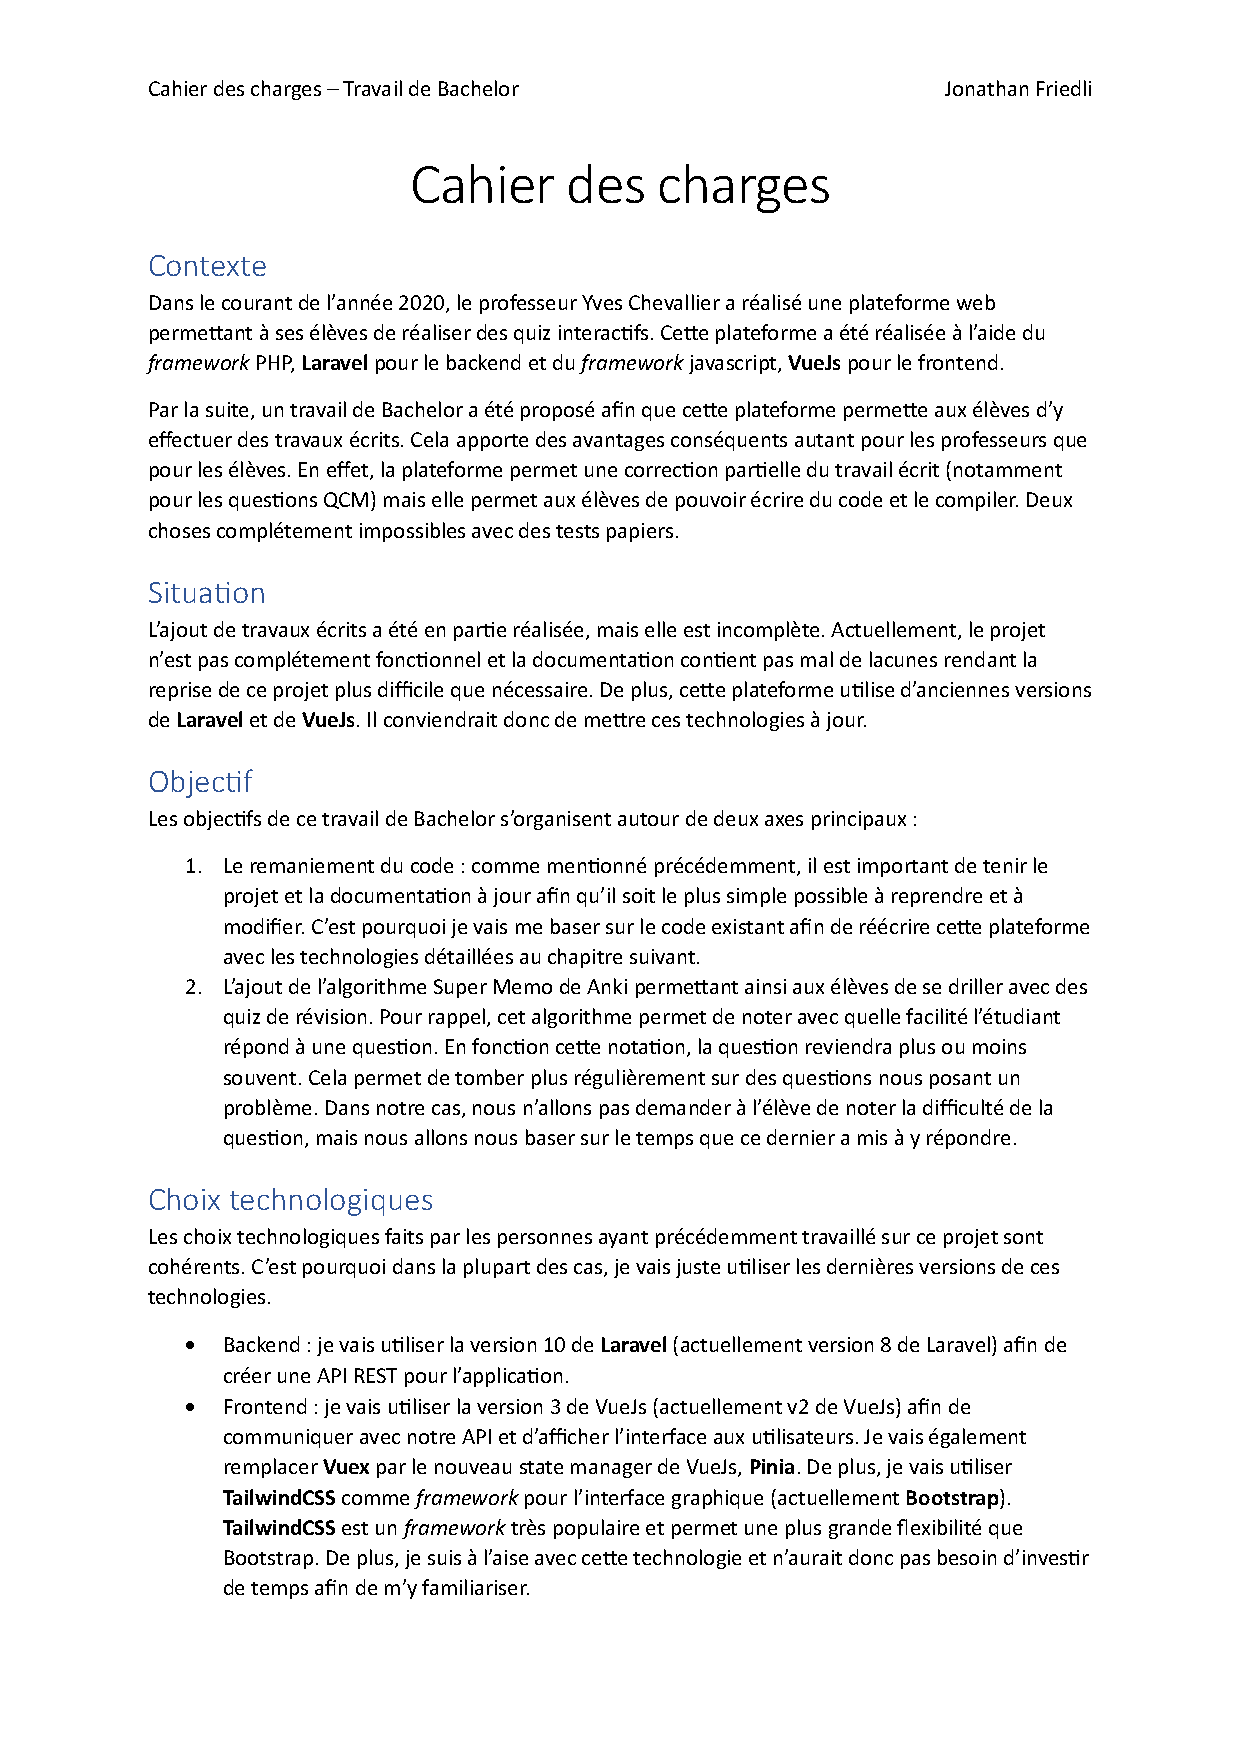
\includepdf[pages=-]{./assets/figures/cdc.pdf}
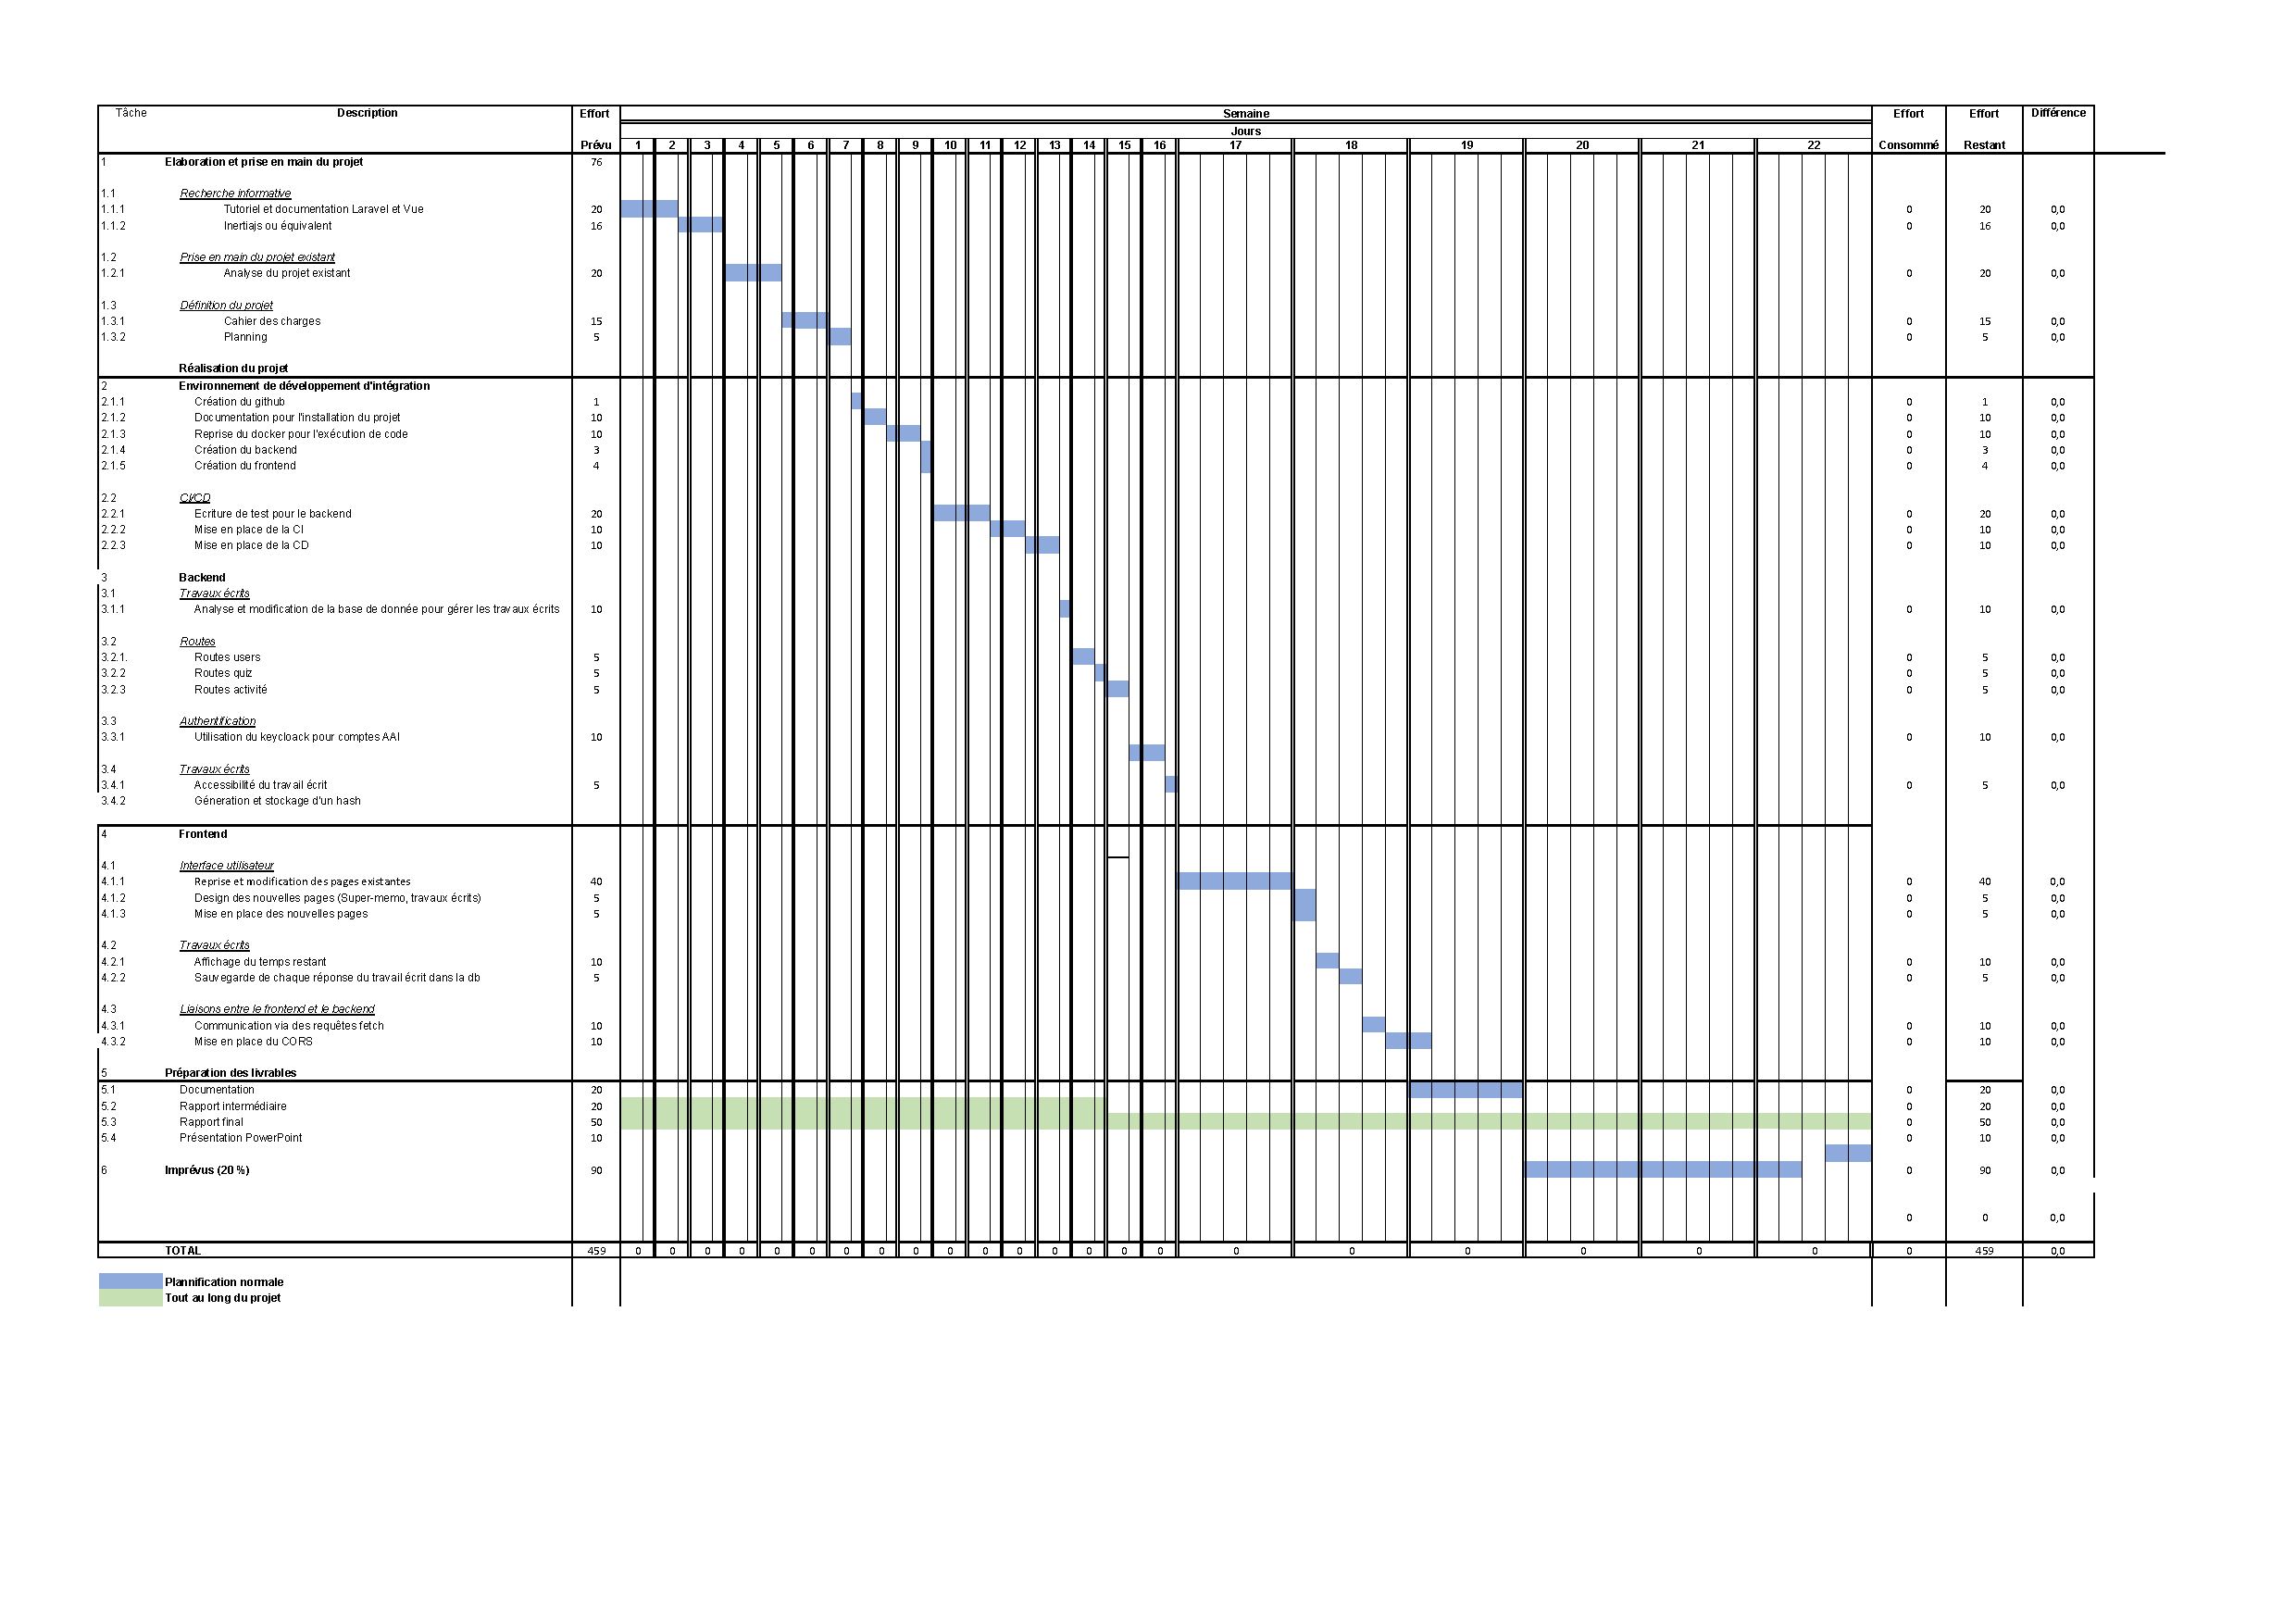
\includepdf[pages=-]{./assets/figures/planif.pdf}
% \addappheadtotoc

%%if
% \chapter{Installation du projet}

% Les annexes n'ont pas un contenu \underline{normatif} mais \underline{descriptif}. Tout contenu annexé ne doit pas être nécessaire à la bonne compréhension du travail.

% Les annexes contiennent généralement :

% \begin{itemize}
%     \item les dessins mécaniques (mises en plan);
%     \item les schémas électriques détaillés;
%     \item des photographies du projet;
%     \item des scripts et des extraits de code source;
%     \item des documents techniques \pex \emph{datasheet};
%     \item des développements mathématiques.
% \end{itemize}
% \section{Sous section}
% \lipsum[1]
%%fi

\let\cleardoublepage\clearpage
\backmatter

\label{glossaire}
\printnoidxglossary
\label{index}
\printindex

% Le colophon est le dernier élément d'un document qui contient des notes de l'auteur concernant la mise en page et l'édition du document : il est parfaitement optionnel.
% \input{colophon.tex}

\end{document}
